% report.tex
% main file for the project report.

\documentclass[a4paper,titlepage,12pt]{scrreprt}

% utf-8
\usepackage{polyglossia}
\setdefaultlanguage[babelshorthands]{ngerman}
\usepackage{fontspec}
\usepackage{pdfpages}

%Needed to wrap text around images, used for personas
\usepackage{wrapfig}

%Used to avoid page breaks with each chapter
\usepackage{etoolbox}
\makeatletter
\patchcmd{\chapter}{\if@openright\cleardoublepage\else\clearpage\fi}{}{}{}
\makeatother

% german names
\usepackage{ngerman}

% colored links
\usepackage{color}
\usepackage[colorlinks=true, citecolor=red] {hyperref}
\definecolor{grey}{rgb}{0.2,0.2,0.2}
\definecolor{orange}{rgb}{1,0.3,0}
\definecolor{turqoise}{rgb}{0,0.7,0.5}

% code listings
\usepackage{listings}
% "define" Scala
\lstdefinelanguage{scala}{
  morekeywords={abstract,case,catch,class,def,%
    do,else,extends,false,final,finally,%
    for,if,implicit,import,match,mixin,%
    new,null,object,override,package,%
    private,protected,requires,return,sealed,%
    super,this,throw,trait,true,try,%
    type,val,var,while,with,yield},
  otherkeywords={=>,<-,<\%,<:,>:,\#,@},
  sensitive=true,
  morecomment=[l]{//},
  morecomment=[n]{/*}{*/},
  morestring=[b]",
  morestring=[b]',
  morestring=[b]"""
}

% Style languages
\lstset{%
	language=Java,
	basicstyle={\ttfamily \small},
	breaklines=true,
	commentstyle=\color{grey},
	keywordstyle=\color{orange},
	numbers=left,
	showspaces=false,
	stringstyle=\color{turqoise},
	xleftmargin=20pt
}

\lstset{%
	language=scala,
	basicstyle={\ttfamily \small},
	breaklines=true,
	commentstyle=\color{grey},
	keywordstyle=\color{orange},
	numbers=left,
	showspaces=false,
	stringstyle=\color{turqoise},
	xleftmargin=20pt
}


% graphics
\usepackage{graphicx}
\graphicspath{{images/}}

% BibTex lib - used for citation
\usepackage{cite}
% fancy headers and footers
\usepackage{fancyhdr}
\pagestyle{fancy}
% clear style
\fancyhead{}
\fancyfoot{}
% new style
\renewcommand{\chaptermark}[1]{%
	\markboth{\thechapter.\ #1}{}
}
\renewcommand{\sectionmark}[1]{%
	\markright{\thesection.\ #1}{}
}
\renewcommand{\headrulewidth}{0.5pt}
\renewcommand{\footrulewidth}{0.5pt}
\fancyhead[LE,RO]{\rightmark}
\fancyhead[LO,RE]{\leftmark}
\fancyfoot[LE,RO]{\thepage}
\fancyfoot[LO,RE]{Projektarbeit T. Kerst \& P. König --- Sommersemester 2016}
\fancypagestyle{plain}{%
	\fancyhf{}
	\renewcommand{\headrulewidth}{0pt}
	\renewcommand{\footrulewidth}{0.5pt}
	\fancyfoot[LE,RO]{\thepage}
	\fancyfoot[LO,RE]{Projektarbeit T. Kerst \& P. König --- Sommersemester 2016}
}

% no indented paragraphs
\usepackage{parskip}

\setkomafont{disposition}{\normalfont\bfseries}

% for verbatiminput
\usepackage{verbatim}

% not yet used
%\input{src/cmd}

\begin{document}

\titlehead{
	
\includegraphics[width=0.9\linewidth]{hska_logo}
}

\title{Ausarbeitung Projektarbeit}
\subtitle{Multithreadingfähiger Mergesort-Algorithmus in Scala mit Visualisierung über eine grafische Oberfläche}
\author{%
	Tobias Kerst \\
	Patrick König
}
\date{Sommersemester 2016}
\publishers{
    \textbf{Dozent:} Prof. Dr. Heiko Körner
}
\maketitle

\clearpage

\begingroup
\hypersetup{linkcolor=black}
\tableofcontents
\endgroup

\clearpage

\chapter{Einleitung}\label{chap:intro}
\section{Motivation}

\section{Scala}
Wir haben uns entschieden, das Programm in Scala zu schreiben, einer Sprache, die bereits schon im Jahr 2001 von Martin Odersky entwickelt wurde, jedoch erst seit kurzem einen großen Bekanntheitsgrad erlangt hat. Grund dafür ist der Hype um die sogenannte \textit{funktionale Programmierung} und das Bedürfnis, Anwendungen nebenläufig zu entwickeln.
Wir möchten nun zu Beginn die Gründe nennen, warum Scala sich als moderne Programmiersprache anbietet, die sogar von Javas Hauptentwickler James Gosling als bevorzugte Java-Alternative betitelt wurde \footnote{James Gosling wurde auf einer Konferenz gefragt, welche Programmiersprache er heutzutage anstelle von Java auf der JVM nutzen würde, worauf er entschieden mit "Scala" antwortete --- \url{http://www.adam-bien.com/roller/abien/entry/java_net_javaone_which_programming}}.

\subsection{Laufzeit-Umgebung}
Scala ist wie Java eine Programmiersprache, die zu Bytecode kompiliert wird. Dieser Bytecode wird dann von der \textit{Java Virtual Machine} (\texttt{JVM}) benutzt um daraus Maschinencode zu erstellen. Die JVM ist mittlerweile auf sehr vielen Rechnern installiert und sogar das Android Betriebssystem setzt auf eine Variante der JVM (\texttt{Dalvik}).

Die JVM hat den großen Vorteil, dass sie mittlerweile seit 20 Jahren aktiv entwickelt wird und die gesamte Java-Umgebung besonders im Enterprise Bereich eingesetzt wird. Das Resultat ist ein sehr stabiles und vor allem perfomantes System, das aus dem heutigen IT-Markt nicht mehr wegzudenken ist.

\subsection{Bibliotheken}
Scala wird also nicht zu irgendeinem Bytecode kompiliert, sondern zu Java-Bytecode, um genau zu sein. Dies hat den großen Vorteil, dass man neben der JVM-Unterstützung auch auf etablierte Java Bibliotheken zugreifen kann. Beispielsweise ist der Einsatz von Google GSON\footnote{Link zu der Projektseite von Google GSON: \url{https://github.com/google/gson}}, das das Serialisieren von Objekten in JSON und zurück ermöglicht, über Scala so möglich, wie über Java.

So ist es dann auch kaum überraschend, dass der Einsatz von den üblichen Java Bibliotheken in Scala möglich ist. Ein Beispiel ist \texttt{JavaFX}, welches seit Java 8 Teil des \textit{Java Development Kit} (\texttt{JDK}) ist.

\subsection{JavaFX und ScalaFX}
\subsubsection{JavaFX}
JavaFX 8 ist der offzielle Nachfolger von Swing. Zu Beginn sollte es eine Scriptssprache werden, jedoch wurde dieser Fokus mit Version 2 aufgegeben und JavaFX wurde zu der GUI Bibliothek, wie man sie heute nutzt. In der aktuellen Version 8 (welcher der direkte Nachfolger von Version 2 ist und wegen der Einbindung in das JDK 8 diesen Versionssprung vollzogen hat), wurde die Bibliothek um wichtige Komponenten erweitert und bietet die folgendenden Vorteile:

\begin{description}
\item[Scene Graph]\hfill\\
JavaFX ist besonders leicht zu entwickeln, da es auf den \texttt{Scene Graph} setzt. Der Scene Graph ist eine Baumstruktur, bei der die Elemente hierachisch angeordnet werden. Elemente im Scene Graph sind vom Type \texttt{Node} ~\cite{ProJavaFX8}. Wenn man also beispielsweise einen Button auf der Bildfläche platzieren möchte, dann hat man ein Button Objekt, welches von \texttt{Node} erbt

\begin{figure}[!htb]
    \centering
      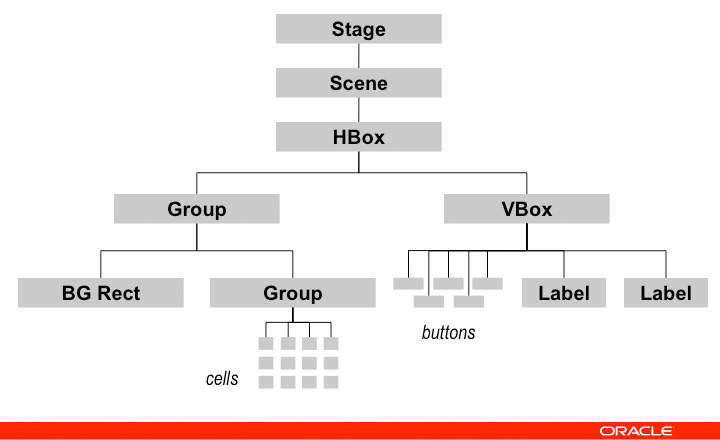
\includegraphics[width=0.75\linewidth]{scene-graph}
    \caption{Darstellung der Baumstruktur im Scene Graph}
    \label{fig:scene-graph}
\end{figure}

Ein Vorteil ist, dass man so Objekte gruppieren kann und dadurch Operationen auf der Gruppe ausführen kann. So wird bei einer Verschiebe-Operation (auch \textit{Translation} genannt) jedes Element in der Gruppe verschoben, was den Code lesbarer und wartbarer macht.\\
Außerdem ist somit eine zum Eltern Element relative Positionierung möglich.

\item[Klares MVC]\hfill\\
Bei JavaFX wird das Konzept für das Design in einer separaten Datei, einer \textbf{FXML} Datei geführt. So muss man das Layout nicht im Code generieren. Im Abschnitt zu FXML~\ref{sec:fxml} wird dies ausführlicher beschrieben.

\item[Styling über CSS]\hfill\\
Neben der Trennung von Ablauf, Logik und Gestaltung nach dem \textit{MVC}-Prinzip, lässt sich das Styling durch eine CSS-ähnliche Syntax durchführen, was das Gestalten von Oberflächen durch Designer ermöglicht. Es wird jedoch eine leicht abgewandelte Syntax verwendet. Das Setzen der Textfarbe auf rot (\texttt{\#ff0000} im RGB-Farbraum) wird durch die CSS-Syntax
\begin{verbatim}
.button: {
  -fx-color: #f00;
}
\end{verbatim}
ermöglicht. Man erkennt, dass das Präfix \texttt{-fx-} vor dem CSS-Befehl steht.

\item[Properties und Bindings]\hfill\\
Das Koppeln von von Eigenschaften einer Klasse an eine andere Klasse ist ein tolles Feature, welches das Entwickeln von komplexen Anwendungen noch weiter vereinfacht. Intern wird das \texttt{Observable}-Interface benutzt, die Komponenten zu aneinander zu binden.

Um Bindings und die dazu benutzten Properties besser zu verstehen, verweisen wir auf die sehr gute Zusammenfassung auf \cite{JavaBeginner-Binding}
\end{description}

\subsubsection{ScalaFX}
\textbf{ScalaFX} ist eine \textit{Domain Specifig Language}\footnote{Bei einer \texttt{DSL} handelt es sich um eine formale Sprache, die ein bestimmtes Problemfeld abdeckt. In dem Fall von ScalaFX handelt es sich um eine \textit{UI DSL}, die als Wrapper um JavaFX gelegt wird.} (\texttt{DSL}) für JavaFX. Als \texttt{DSL} bietet ScalaFX syntaktischen Zucker für die JavaFX--Bibliothek, und die folgenden Vorteile:

\begin{description}
\item[Lesbare Bind-Ausdrücke]\hfill\\
Binding und Properties gehören zu den tollen Funktionen, die JavaFX bietet, jedoch ist die Syntax teilweise sehr umständlich.
\paragraph{Beispiel:} Wenn man 3 Rechtecke hat (\texttt{rect1}, \texttt{rect2} und \texttt{reckt3}) und man möchte, dass das Rechteck \texttt{rect1} so hoch ist, wie \texttt{rect2} und \texttt{rect3}, dann bindet man die Höhe von \texttt{rect1} an die summierte Höhe von \texttt{rect2} und \texttt{rect3}.

\underline{Scala}:
\begin{lstlisting}[language=scala,caption=Scala Beispiel Code für natürliche Bindings,numbers=none]
rect1.height <== rect2.height + rect3.height
\end{lstlisting}

\underline{Java}:
\begin{lstlisting}[language=Java,caption=Das selbe Beispiel in Java,numbers=none]
rect1.heightProperty().bind(rect2.heightProperty().add(rect3.heightProperty()))
\end{lstlisting}

Der Scala Code ist wesentlich intuitiver und lesbarer, was genau der Sinn dieser \texttt{DSL} ist. Das Beispiel stammt aus \cite{ProJavaFX8} (Seite 574f.).

\item[Angepasste Animations Syntax]\hfill\\
Da Animationen ein wichtiger Bestandteil von JavaFX sind, wurde die Syntax wesentlich verbessert. Auch hier möchten wir uns an \cite{ProJavaFX8} halten und Scala Code mit Java Code vergleichen.

\underline{Scala}:
\begin{lstlisting}[language=scala,caption=Scala Beispiel für eine einface Animation,numbers=none]
Timeline(at (3 s) {radius -> 0}).play()
\end{lstlisting}

\underline{Java}:
\begin{lstlisting}[language=Java,caption=Das selbe Beispiel in Java,numbers=none]
KeyValue collapse = new KeyValue(circle.radiusProperty(), 0);
new Timeline(new KeyFrame(Duration.seconds(3), collapse)).play();
\end{lstlisting}

\item[Typsichere APIs]\hfill\\
Ein Vorteil von Scala, wie wir noch kennen lernen werden, ist dass die Sprache \textit{statisch typisiert} ist. ScalaFX ist garantiert \textit{typsicher}, was zur Folge hat, dass Fehler bereits beim Kompilieren auftreten und nicht erst zur Laufzeit zu Fehlern führen wird. ~\cite{TypesAndProgrammingLanguages}

\item[Interoperabilität zwischen ScalaFX und JavaFX]\hfill\\
ScalaFX liegt wie ein Wrapper um JavaFX und bietet Funktionen an, die die Arbeit mit JavaFX erleichtern. Dies wird dadurch vereinfacht, dass man ganz einfach zwischen JavaFX und ScalaFX wechseln kann. Ein besonders hilfreiches Konzept sind hierbei \textit{Implizite Konvertierungen}. So kann man beispielsweise eine \texttt{javafx.scene.Shape.button} an eine Methode übergeben, die ein \texttt{scalafx.scene.Shape.button} als Argument erwartet.
\end{description}

Da es sich bei ScalaFX primär um syntaktische Verbesserungen handelt, kann man argumentieren, dass die Benutzung obsolet ist. Wir haben uns bewusst für die Integration entschieden, da wir näher an der Scala Syntax bleiben wollten und die Lesbarkeit von Source-Code für uns ein wichtiger Aspekt ist\footnote{Eine Interessante Diskussion zu diesem Thema findet man auch hier \cite{StackoverflowDiscussionScalaFX}}.
\subsection{FXML}\label{sec:fxml}

\section{Ziele \& Fragen}
\section{Methodische Vorgehensweise}

\clearpage

\chapter{Scala}
Wir haben uns entschieden, das Programm in Scala zu schreiben, einer Sprache, die bereits schon im Jahr 2001 von Martin Odersky\footnote{\url{https://de.wikipedia.org/wiki/Martin_Odersky}} entwickelt wurde, jedoch erst seit Kurzem einen großen Bekanntheitsgrad erlangt hat. Grund dafür ist der Hype um die sogenannte \textit{funktionale Programmierung} und das Bedürfnis, Anwendungen nebenläufig zu entwickeln.\\
Wir möchten nun zu Beginn die Gründe nennen, warum Scala sich als moderne Programmiersprache anbietet, die sogar von Javas Hauptentwickler James Gosling\footnote{\url{https://de.wikipedia.org/wiki/James_Gosling}} als bevorzugte Java-Alternative betitelt wurde \footnote{James Gosling wurde auf einer Konferenz gefragt, welche Programmiersprache er heutzutage anstelle von Java auf der JVM nutzen würde, worauf er entschieden mit ``Scala'' antwortete --- \url{http://www.adam-bien.com/roller/abien/entry/java_net_javaone_which_programming}}.

\section{Laufzeit-Umgebung}
Scala ist wie Java eine Programmiersprache, die zu Bytecode kompiliert wird. Dieser Bytecode wird dann von der \textit{Java Virtual Machine} (\texttt{JVM}) benutzt, um daraus Maschinencode zu erstellen. Die JVM ist mittlerweile auf sehr vielen Rechnern installiert und sogar das Android Betriebssystem setzt auf eine Variante der JVM (\texttt{Dalvik}).

Die JVM hat den großen Vorteil, dass sie mittlerweile seit 20 Jahren aktiv entwickelt wird und die gesamte Java-Umgebung besonders im Enterprise--Bereich eingesetzt wird. Das Resultat ist ein sehr stabiles und vor allem perfomantes System, das aus dem heutigen IT-Markt nicht mehr wegzudenken ist.

\section{Bibliotheken}
Scala wird also nicht zu irgendeinem Bytecode kompiliert, sondern zu Java-Bytecode, um genau zu sein. Dies hat den großen Vorteil, dass man neben der JVM-Unterstützung auch auf etablierte Java Bibliotheken zugreifen kann. Beispielsweise ist der Einsatz von Google GSON\footnote{Link zu der Projektseite von Google GSON: \url{https://github.com/google/gson}}, das das Serialisieren von Objekten in JSON und zurück ermöglicht, über Scala so möglich, wie auch über Java.

So ist es dann auch kaum überraschend, dass der Einsatz von den üblichen Java Bibliotheken in Scala möglich ist. Ein Beispiel ist \texttt{JavaFX}, welches seit Java 8 Teil des \textit{Java Development Kit} (\texttt{JDK}) ist.

\section{JavaFX und ScalaFX}
Um die Oberfläche (User Interface) zu gestalten, nutzt man heute Bibliotheken, die meistens so komplex sind, dass ihnen ganze Werke gewidmet werden. Wir haben uns für JavaFX entschieden, welches durch den Wrapper ScalaFX angesprochen wird. Was diese Bibliotheken machen und auszeichnet, wird in den folgenden Abschnitten erklärt.

\subsection{JavaFX}
JavaFX 8 ist der offzielle Nachfolger von Swing. Zu Beginn sollte es eine Scriptssprache werden, jedoch wurde dieser Fokus mit Version 2 aufgegeben und JavaFX wurde zu der GUI Bibliothek, wie man sie heute nutzt. In der aktuellen Version 8 (welcher der direkte Nachfolger von Version 2 ist und wegen der Einbindung in das JDK 8 diesen Versionssprung vollzogen hat), wurde die Bibliothek um wichtige Komponenten erweitert und bietet die folgendenden Vorteile:

\begin{description}
\item[Scene Graph]\hfill\\
JavaFX ist besonders leicht zu entwickeln, da es auf den \texttt{Scene Graph} setzt. Der \texttt{Scene Graph} ist eine Baumstruktur, bei der die Elemente hierachisch angeordnet werden. Elemente im \texttt{Scene Graph} sind vom Type \texttt{Node} ~\cite{ProJavaFX8}. Wenn man also beispielsweise einen Button auf der Bildfläche platzieren möchte, dann hat man ein Button Objekt, welches von \texttt{Node} erbt.

\begin{figure}[!htb]
    \centering
      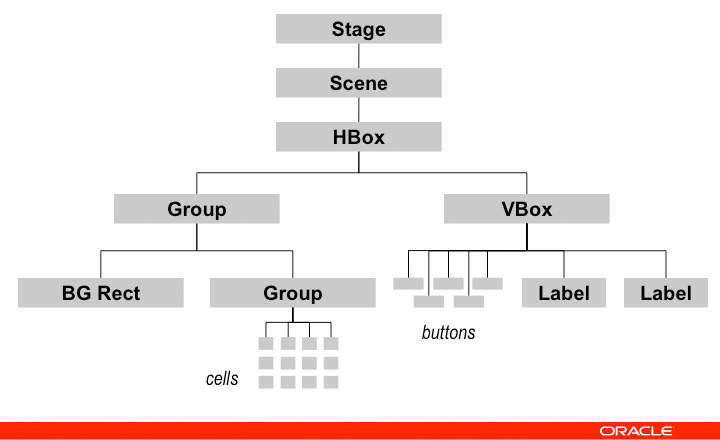
\includegraphics[width=0.75\linewidth]{scene-graph}
    \caption{Darstellung der Baumstruktur im \texttt{Scene Graph}}{\url{http://www.smarks.org/svjugfx20100414/flood.html}}
    \label{fig:scene-graph}
\end{figure}

Ein Vorteil ist, dass man so Objekte gruppieren kann und dadurch Operationen auf der Gruppe ausführen kann. So wird bei einer Verschiebe-Operation (auch \textit{Translation} genannt) jedes Element in der Gruppe verschoben, was den Code lesbarer und wartbarer macht.\\
Außerdem ist somit eine zum Eltern Element relative Positionierung möglich.

\item[Klares MVC]\hfill\\
Bei JavaFX wird das Konzept für das Design in einer separaten Datei, einer \textbf{FXML} Datei geführt. So muss man das Layout nicht im Code generieren. Im Abschnitt zu FXML~\ref{sec:fxml} wird dies ausführlicher beschrieben.

\item[Styling über CSS]\hfill\\
Neben der Trennung von Ablauf, Logik und Gestaltung nach dem \textit{MVC}-Prinzip, lässt sich das Styling durch eine CSS-ähnliche Syntax durchführen, was das Gestalten von Oberflächen durch Designer ermöglicht. Es wird jedoch eine leicht abgewandelte Syntax verwendet. Das Setzen der Textfarbe auf rot (\texttt{\#ff0000} im RGB-Farbraum) wird durch die CSS-Syntax
\begin{verbatim}
.button: {
  -fx-color: #f00;
}
\end{verbatim}
ermöglicht. Man erkennt, dass das Präfix \texttt{-fx-} vor dem CSS-Befehl steht.

\item[Properties und Bindings]\hfill\\
Das Koppeln von Eigenschaften einer Klasse an eine andere Klasse ist ein tolles Feature, welches das Entwickeln von komplexen Anwendungen noch weiter vereinfacht. Intern wird das \texttt{Observable}-Interface benutzt, die Komponenten aneinander zu binden.

Um Bindings und die dazu benutzten Properties besser zu verstehen, verweisen wir auf die sehr gute Zusammenfassung von \cite{JavaBeginner-Binding}.
\end{description}

\subsection{ScalaFX}
ScalaFX ist eine \textit{Domain Specifig Language}\footnote{Bei einer \texttt{DSL} handelt es sich um eine formale Sprache, die ein bestimmtes Problemfeld abdeckt. In dem Fall von ScalaFX handelt es sich um eine \textit{UI DSL}, die als Wrapper um JavaFX gelegt wird.} (\texttt{DSL}) für JavaFX. Als \texttt{DSL} bietet ScalaFX syntaktischen Zucker für die JavaFX--Bibliothek, und die folgenden Vorteile:

\begin{description}
\item[Lesbare Bind-Ausdrücke]\hfill\\
Binding und Properties gehören zu den tollen Funktionen, die JavaFX bietet, jedoch ist die Syntax teilweise sehr umständlich.
\paragraph{Beispiel:} Wenn man 3 Rechtecke hat (\texttt{rect1}, \texttt{rect2} und \texttt{reckt3}) und man möchte, dass das Rechteck \texttt{rect1} so hoch ist, wie \texttt{rect2} und \texttt{rect3}, dann bindet man die Höhe von \texttt{rect1} an die summierte Höhe von \texttt{rect2} und \texttt{rect3}.

\underline{Scala}:
\begin{lstlisting}[language=scala,caption=Scala Beispiel Code für natürliche Bindings,numbers=none]
rect1.height <== rect2.height + rect3.height
\end{lstlisting}

\underline{Java}:
\begin{lstlisting}[language=Java,caption=Das selbe Beispiel in Java,numbers=none]
rect1.heightProperty().bind(rect2.heightProperty().add(rect3.heightProperty()))
\end{lstlisting}

Der Scala Code ist wesentlich intuitiver und lesbarer, was genau der Sinn dieser \texttt{DSL} ist. Das Beispiel stammt aus \cite{ProJavaFX8} (Seite 574f.).

\item[Angepasste Animations--Syntax]\hfill\\
Da Animationen ein wichtiger Bestandteil von JavaFX sind, wurde die Syntax wesentlich verbessert. Auch hier möchten wir uns an \cite{ProJavaFX8} halten und Scala Code mit Java Code vergleichen.

\underline{Scala}:
\begin{lstlisting}[language=scala,caption=Scala Beispiel für eine einface Animation,numbers=none]
Timeline(at (3 s) {radius -> 0}).play()
\end{lstlisting}

\underline{Java}:
\begin{lstlisting}[language=Java,caption=Das selbe Beispiel in Java,numbers=none]
KeyValue collapse = new KeyValue(circle.radiusProperty(),0);
new Timeline(new KeyFrame(Duration.seconds(3), collapse))
  .play();
\end{lstlisting}

\item[Typsichere APIs]\hfill\\
Ein Vorteil von Scala, wie wir noch kennen lernen werden, ist, dass die Sprache \textit{statisch typisiert} ist. ScalaFX ist garantiert \textit{typsicher}, was zur Folge hat, dass Fehler bereits beim Kompilieren auftreten und nicht erst zur Laufzeit zu Fehlern führen wird. ~\cite{TypesAndProgrammingLanguages}

\item[Interoperabilität zwischen ScalaFX und JavaFX]\hfill\\
ScalaFX liegt wie ein Wrapper um JavaFX und bietet Funktionen an, die die Arbeit mit JavaFX erleichtern. Dies wird dadurch vereinfacht, dass man ganz einfach zwischen JavaFX und ScalaFX wechseln kann. Ein besonders hilfreiches Konzept sind hierbei \textit{Implizite Konvertierungen}. So kann man beispielsweise eine \texttt{javafx"".scene"".Shape"".button} an eine Methode übergeben, die ein \texttt{scalafx"".scene"".Shape"".button} als Argument erwartet.
\end{description}

Da es sich bei ScalaFX primär um syntaktische Verbesserungen handelt, kann man argumentieren, dass die Benutzung obsolet ist. Wir haben uns bewusst für die Integration entschieden, da wir näher an der Scala Syntax bleiben wollten und die Lesbarkeit von Source-Code für uns ein wichtiger Aspekt ist\footnote{Eine Interessante Diskussion zu diesem Thema findet man auch hier \url{http://stackoverflow.com/a/22744881}}.


\subsection{FXML}\label{sec:fxml}
Wenn man sich mit den Entwicklung von Swing auskennt, dann weiß man, dass man alle darstellbaren Objekte im Code selber generiert und gestaltet. Möchte man diese dann später ändern, so muss man sich mit dem Programmcode auseinander setzen und hier die Syntax nachvollziehen und Änderungen über die Programmiersprache vornehmen.

Dieser Ansatz ist in JavaFX auch möglich, jedoch hat dies den Nachteil, dass die Oberfläche durch den teilweise umständlichen Programmierstil beschrieben wird. Außerdem müssen sich Oberflächen-Gestalter in die Programmiersprache einarbeiten.\\
FXML ist eine auf \texttt{XML} basierende Sprache, dass die Struktur des Layouts beschreibt. Man kann das FXML Layout ganz einfach auslagern, also in einer separaten Datei speichern, sodass Anwendungs-Logik und die Präsentationsschicht getrennt sind, so wie im \texttt{Model-View-Control} Pattern gefordert.

Dadurch, dass das Layout über den Scene\textbf{graph} organisiert wird, bietet sich XML durch seine verschachtelten Tags an, diese Knotenstruktur abzubilden. Somit wird diese Struktur auch gleichzeitig \textbf{transparent}.\\
FXML wird nicht kompiliert, somit können Änderungen ohne vorheriges Rekompilieren direkt getestet werden.\\
Ein großer Vorteil ist, dass man einzelnen Knoten \texttt{ID}s und \texttt{Class}es zuteilen kann, wie in HTML. Diese lassen sich dann über CSS stylen. Hierbei wird eine leicht veränderte CSS-Syntax verwendet, aber jeder der sich in der Webgestaltung auskennt, wird sich hier schnell zurecht finden. Neben dem Stylen von Elementen ist die \textbf{Lokalisierung} des Inhalts heutzutage auch extrem wichtig, da der Softwaremarkt mittlerweile kaum mehr auf einen Sprachraum beschränkt ist. Hier bietet FXML eingebaute Features, die diese Lokalisierung sehr einfach ermöglichen.\\
Und da JavaFX das Laden und verarbeiten von FXML Dateien erlaubt, kann man auch mit anderen JVM--Sprachen, wie in unserem Fall Scala, FXML nutzen. Wir haben jedoch eine zusätzliche Library genutzt, die das Benutzen und Arbeiten mit FXML Dateien erleichtert: ScalaFXML~\cite{ScalaFXML}.

Zuletzt muss man in Verbindung mit FXML noch den Scene Builder\footnote{Der Scene Builder ist mittlerweile Open Source und kann hier herunter geladen werden \url{http://gluonhq.com/labs/scene-builder/}. Weitere Informationen findet man noch auf der mittlerweile archivierten Oracle Seite unter \url{http://www.oracle.com/technetwork/java/javase/downloads/javafxscenebuilder-info-2157684.html}} nennen. Dieses Tool erleichtert die Gestaltung von einfachen User Interfaces, indem Elemente per Drag \& Drop platziert werden können und man somit eine Oberfläche gestalten kann, ohne sich genauer mit dem FXML Code auseinander setzen zu müssen. Das Programm hat uns am Anfang geholfen, die Syntax besser zu verstehen und die Elemente besser zu platzieren. Da wir in unserer Arbeit jedoch immer öfter Kleinigkeiten im Layout anpassen mussten, haben wir im Verlauf immer mehr auf den Scene Builder verzichtet, da die Anpassung einer ID, oder Größe oder das Einfügen eine Buttons händisch tatsächlich schnell geht und der Scene Builder nicht fehlerfrei funktionierte. Bei uns wurde die Menüzeile des Scene-Builders, die man beispielsweise nutzen kann, um von dort aus das Layout als native Anwendung ohne Logik zu testen,  durch das Menü unserer Anwendung überschrieben \footnote{Der Fehler wird hier beschrieben: \url{https://bugs.openjdk.java.net/browse/JDK-8089659}. Wir haben das Tag \texttt{useSystemMenuBar} genutzt, um auf OSX die native Menüzeile zu nutzen, was das Layout natürlicher macht.}.

\section{Grundlegendes und Syntax}
Die Programmiersprache Scala ist sehr komplex und die Sprache hier vorzustellen und zu erklären würde den Umfang dieser Ausarbeitung sprengen. Dennoch möchten wir einige Grundlegende Spracheigenschaften vorstellen, sodass man den später vorgestellten Code besser nachvollziehen kann.\\
Man kann zwar Scala Code schreiben, der sehr an Java Code erinnert, jedoch wird davon abgeraten. Einer der grundlegenden Ansätze\footnote{Siehe: \url{http://www.scala-lang.org/documentation/getting-started.html}} ist, dass man sich die elementaren Konzepte von Scala verinnerlicht und Code schreibt, der funktioniert. Man kann dann immer noch die komplexeren Eigenschaften der Sprache lernen.

Da dies das erste Programm ist, das wir in Scala geschrieben haben, kann man bestimmt viele Sachen besser machen, wenn man entsprechend Erfahrung hat. Dennoch haben wir probiert, viele der tollen Features zu nutzen, die Scala bietet.

Viele der folgenden Beispiele kann man in der \textbf{REPL} (\texttt{Read-Evaluate-Print-Loop}) testen. Die REPL ist so etwas wie eine interaktive Console, in der man Scala Code testen und ausprobieren kann. Da wir diese für unsere Projektarbeit nicht direkt benötigten, aber eine tolle Möglichkeit darstellt um Scala Code zu testen, verweisen wir auf die tolle Beschreibung von \cite{GettingStartedWithTheScalaREPL}

\subsection{Typinferenz}
Scala ist eine statisch typisierte Sprache. Das bedeutet, dass eine Variable von einem Typ ist, der sich auch nicht ändert. In Java gibt man den Typ bei der Deklaration direkt mit an. Wenn man Beispielsweise einen Variable \texttt{helloWorld} vom Type \texttt{String} hat, die den Wert \texttt{Hello World} hat, dann wird dies wie folgt angegeben:

\begin{lstlisting}[language=Java,numbers=none]
String helloWorld = "Hello World";
\end{lstlisting}

In Scala kann man den Typ weglassen, den die Variable hat, dieser wird vom Compiler beim Kompilieren ausgewertet. Es reicht also, wenn man

\begin{lstlisting}[language=Scala,numbers=none]
val helloWorld = "Hello World"
\end{lstlisting}

schreibt.\\
Wenn man möchte, so kann man den Typ dennoch mit angeben, das sieht dann wie folgt aus:

\begin{lstlisting}[language=Scala,numbers=none]
val helloWorld: String = "Hello World"
\end{lstlisting}

In den obigen Beispielen fällt auf, dass es ein Schlüsselwort gibt, das es in Java so nicht gibt: \texttt{val}. Außerdem muss man kein Semikolon an das Ende der Zeilen machen. Wie so oft in Scala gilt für das Semikolon: Muss man nicht, kann man aber.\\
Was es mit dem Schlüsselwort \texttt{val} auf sich hat, möchten wir im nächsten Abschnitt aufzeigen.

\subsection{Values und Variablen}
Das \texttt{val} steht für einen Value, also einen unveränderlichen Wert. Scala ist eine funktionale Programmiersprache. Einer der wichtigen Ansätze hierbei ist die \textit{Immuntability}, also die \textit{Unveränderlichkeit} von Werten. Man möchte bei nebenläufigen Operationen keine Werte haben, die von anderen Threads verändert werden können. Um dies zu vermeiden, benutzt man unveränderliche Werte, also \textbf{Values}. Dies entspricht einer \texttt{final}-Variable in Java.\\
Das Code-Fragment

\begin{lstlisting}[language=Scala,numbers=none]
val number = 1
number = 2
\end{lstlisting}

führt also zu dem Fehler:
\begin{verbatim}
error: reassignment to val
\end{verbatim}

An dieser Stelle benötigt man also eine Variable \texttt{var}:

\begin{lstlisting}[language=Scala,numbers=none]
var number = 1
number = 2
\end{lstlisting}

\subsection{Methoden}
Methoden werden ähnlich wie in Java geschrieben. Sie haben einen Rückgabetype und eine ParameterListe. Wir wollen uns im folgenden eine sehr einfache Methode angucken:

\begin{lstlisting}[language=Scala]
def isLarge(value: Int): Boolean = {
  if (value > 15)
    true
  else
    false
}
\end{lstlisting}

Die Methode mit dem Namen \texttt{isLarge} nimmt also als Parameter einen \texttt{Integer}, den man mit dem Namen \texttt{value} anspricht. Die Methode hat Rückgabetyp \texttt{Boolean}.

Die Methode zeigt auch schon einige Besonderheiten an Scala. Man erkennt, dass das Schlüsselwort \texttt{return} nicht angegeben werden muss. In Java würde man \texttt{return true} und \texttt{return false} schreiben müssen \footnote{Man kann if Statements wie einen ternären Operator nutzen, siehe: \cite{ScalaCookbook} Section 3.6 --- \textit{Using the if Construct Like a Ternary Operator}} \footnote{Return Statements sollten vermieden werden, wie in \cite{ScalaInDepth} Section 2.2.1 --- \textit{Don't use return} beschrieben}. Dies hat den Hintergrund, dass \textbf{jeder Ausdruck ausgewertet wird} und somit etwas zurück gegeben wird. Wenn man nichts zurückgeben möchte, so gibt man \texttt{Unit} an. Unit gibt an, dass man mit dem Ergebnis, das zurückgegeben wird, nichts anfangen kann und kommt dem \texttt{void} in Java nahe. Beispielsweise die \texttt{println()} Methode hat den Rückgabetyp \texttt{Unit}.

Um das obige Beispiel noch klarer zu machen, speichern wir den von dem If-Statement zurückgegebenen Wert in einem Value, den wir dann zurück geben werden:

\begin{lstlisting}[language=Scala]
def isLarge2(value: Int): Boolean = {
  val isValueLarger = (if (value > 15) true else false)

  isValueLarger
}
\end{lstlisting}

Die beiden Methoden machen beide das Selbe. Wenn wir die Methode in der \texttt{REPL} testen, bekommen wir folgendes Ergebnis:

\begin{verbatim}
  scala> def isLarge(value: Int): Boolean = {
       |   val isValueLarger = (if (value > 15) true else false)
       |
       |   isValueLarger
       | }
  isLarge: (value: Int)Boolean

  scala> isLarge(9)
  res0: Boolean = false

  scala> isLarge(20)
  res1: Boolean = true
\end{verbatim}

Wir werden die Methode \texttt{isLarge} im weiterhin benutzen, um die Funktionen von Scala hervorzuheben.

\subsection{Strings}

Das Arbeiten mit Strings in Scala ist sehr einfach und es gibt einige sehr nützliche Funktionen, die dafür sorgen, dass der Code nicht nur lesbarer, sondern auch leichter zu warten ist.

Das Konkatenieren von Strings und Variablen in Java ist sehr praktisch und einfach, man fügt diese einfach durch ein \texttt{+} Zeichen aneinander.

\begin{lstlisting}[language=Java,numbers=none]
System.out.println("Is the number " + number + " a large number: " isLarge(number));
\end{lstlisting}

In Scala muss man sich keine Gedanken mehr um das Konkatenieren an sich machen, der gleiche Code wie oben sieht so aus:

\begin{lstlisting}[language=Scala,numbers=none]
println(s"Is the number $number a large number: ${isLarge(number)}")
\end{lstlisting}

Das Weglassen von \texttt{System.out} ist kein Fehler, sondern ein Scala nicht nötig. Durch das Voransetzen von \texttt{s} an den String, kann man Variablen durch \texttt{\$} ganz einfach einsetzen. Ausdrücke werden durch \texttt{\$\{\}} eingefügt, müssen also geklammert werden.

\subsubsection{Mehrzeilige Strings mit Sonderzeichen}
Ein weiteres tolles Feature ist, dass man mehrzeilige Strings nicht manuell umbrechen muss. Durch das Setzen von drei Anführungszeichen zu Beginn des Strings, kann man den String einfach umbrechen:

\begin{lstlisting}[language=Scala]
val multiLineString = """This
     |is
     |an
     |example""".stripMargin
println(multiLineString)
\end{lstlisting}

Dies ergibt die Ausgabe:

\begin{verbatim}
This
is
an
example
\end{verbatim}

Eine tolle Beschreibung für diese Funktionalität gibt es in \cite{ScalaCookbook} unter Section 1.2.

Eine weitere syntaktische Neuerung ist, dass die Methode \texttt{stripMargin()} ohne die Klammern aufgerufen wird. Dies ist in Scala möglich, wenn eine Methode keine Argumente erwartet.

Tatsächlich ist es möglich, dass man sogar den Punkt zwischen dem String (also dem Objekt) und der Methode weglässt. Dies bezeichnet man als \textit{Postfix Operator Notation}, ein Feature, was Code teilweise sehr lesbar und schön macht, aber auch zu unerwartetem Verhalten führen kann.\footnote{Diese Stackoverflow Diskussion klärt einige dieser Fragen, setzt jedoch voraus, dass man sich mit der Scala Syntax auskennt: \url{http://stackoverflow.com/questions/13011204/scalas-postfix-ops}}

\subsection{Getter \& Setter}\label{sec:getter-and-setter}
Die Nutzung von Getter-- und Setter--Methoden Zugriff auf die Attribute eines Objekts ist gang und gäbe in Java. In Scala wird auf die Felder so zugegriffen, als wären diese public, obwohl dies nicht der Fall ist. Scala generiert beim Kompilieren die Methoden, die den Zugriff auf die Variablen erlauben. Ein Beispiel\footnote{Das Beispiel stammt von \url{http://dustinmartin.net/getters-and-setters-in-scala/}} soll dies veranschaulichen:

\begin{lstlisting}[language=Scala, caption=Beispiel Klasse Person]
class Person() {
  var name = ""
  var age = 0
}
\end{lstlisting}

Da die Klasse keine Methoden hat, könnte man meinen, dass der Zugriff auf \texttt{name} und \texttt{age} nicht möglich ist. Jedoch wurden die Getter-- und Setter--Methoden von Scala automatisch erstellt und man kann nun auf die Felder zugreifen:

\begin{lstlisting}[language=Scala]
person = new Person()

println(person.age)
println(person.name)
\end{lstlisting}

Man kann die Getter und Setter auch überschreiben, siehe hierzu \cite{ScalaCookbook} Section 4.6 und die Quelle dieses Beispiels.

\subsection{For--Schleifen}\label{sec:for-loops}

Schleifen sind ein elementares Konstrukt aus der Programmierung. Bei den For--Schleifen wird dabei meistens eine Zählvariable benutzt, die bis zu einem gewissen Wert zählt und auf die man währenddessen zugreifen kann. Ein klassisches Beispiel ist das Befüllen eines Arrays mit Werten.

\begin{lstlisting}[language=Java,caption=Typische For--Schleife aus der Java Programmierung]
for (int i = 0; i <= array.length; i++) {
  array[i] = i * i;
}
\end{lstlisting}

In dem obigen Beispiel wird das Quadrat vom Index als Wert in dem Array gespeichert. Dabei wird jedoch im Schleifen--Kopf manuell geprüft, ob das Ende des Arrays erreicht ist Um typische Fehler zu vermeiden (beispielsweise \texttt{ArrayIndexOutOfBoundsException}), wurden Iteratoren eingeführt und man durchläuft damit Listen etc. durch For-Each Schleifen. Wenn man jedoch einen Index-Zugriff ermöglichen will, so benötigt man wieder eine Zählvariable.

\begin{lstlisting}[language=Java]
int i = 0;
for (int element : array) {
  System.out.println(i + ": " + element); // Gibt Index und enthaltenes Element aus
  i++;
}
\end{lstlisting}

Da die Zählvariable \texttt{i} somit \textit{variabel} sein müsste, gibt es in Scala einen anderen Ansatz. Man kann durch ein Schleifenkonstrukt wie folgt, die obige Ausgabe erreichen:

\begin{lstlisting}[language=Scala]
val array = new Array(1,2,3,4,5,6)
for (i <- 0 until array.length) {
  println(s"$i: ${array(i)"})
}
\end{lstlisting}

Wie man erkennt, greift man nicht mehr über \texttt{array[i]} auf ein Element in dem Array zu, sondern über \texttt{array(i)}. Ansonsten zählt man die i Variable hoch. Man kann auch eine For-Each Schleife kreiren, so wird aus dem Beispiel oben:

\begin{lstlisting}[language=Scala,caption=For--Each in Scala]
var i = 0
for (element <- array) {
  println(s"$i: $element)
  i += 1
}
\end{lstlisting}

Die Syntax sollte nun nicht mehr überraschen, man nimmt jedes Element aus dem Array und gibt die Anzahl aus. Eine schönere Methode, die wir auch in unserer Projektarbeit öfter benutzt haben, ist sich die Zählvariable generieren zu lassen. Hierzu nutzt man die \texttt{zipWithIndex} Methode.

\begin{lstlisting}[language=Scala]
for ((element, index) <- array.zipWithIndex) {
  println(s"$index: $element")
}
\end{lstlisting}

Nun haben wir einige Schleifen-Konstrukte kennen gelernt, jedoch nutzt man in Scala üblicherweise die \texttt{foreach}--Methode, die direkt in der Collection angeboten wird. Hier macht sich bemerkbar, dass Scala eine funktionale Programmiersprache ist. Man übergibt an die \texttt{foreach}--Methode nämlich eine Funktion, die jedes Mal ausgeführt wird. Am besten betrachtet man ein Beispiel, um mit der Syntax vertraut zu werden.

\begin{lstlisting}[language=Scala]
val array = new Array(1,2,3,4,5,6)
array.foreach(e: Int => println(e))
\end{lstlisting}

Hier wird die an die For-Each Methode die Funktion

\begin{lstlisting}[language=Scala,numbers=none]
e: Int => println(e)
\end{lstlisting}

übergeben. Da in dem Array Elemente vom Typ enthalten sind, nimmt die Funktion Werte \texttt{e} von Typ \texttt{Int}. Für diese Werte wird dann die Funktion \texttt{println(e)} aufgerufen. Man kann diesen Ausdruck auch in einem Value speichern und so an die \texttt{forearch}--Methode übergeben.

\begin{lstlisting}[language=Scala,numbers=none]
val printElements = {e: Int => println(e)}
\end{lstlisting}

Nun gibt es in Scala noch einige Möglichkeiten, den Code weiter zu minimieren und somit lesbarer zu machen. So kann man die Typangabe von \texttt{e: Int} weglassen und lediglich \texttt{e} schreiben, da die \texttt{foreach}--Methode auf einer Liste von \texttt{Int}s aufgerufen wird.

\begin{lstlisting}[language=Scala,numbers=none]
array.foreach(e => println(e))
\end{lstlisting}

Und da klar ist, auf welches Element zugegriffen wird, kann man den Variablennamen ganz weglassen und einfach auf das Element zugreifen mit \texttt{\_}. Das sieht das so aus:

\begin{lstlisting}[language=Scala,numbers=none]
array.foreach(println(_))
\end{lstlisting}

Benötigt man den Index, dann kann man auch hier wieder die \texttt{zipWithIndex} Methode benutzen:

\begin{lstlisting}[language=Scala,numbers=none]
array.zipWithIndex.foreach(e => println(s"${e._2}: ${e._1}"))
\end{lstlisting}

Was es mit dem \texttt{e.\_2} und \texttt{e.\_} auf sich hat, sehen wir im kommenden Abschnitt.

\subsection{Tupel}
Tupel sind ein in Scala eingebautes Feature, welches bei Java seit jeher vermisst wird. In einem Tupel werden zwei, oder mehr Elemente abgespeichert, auf die man im Anschluss zugreifen möchte. Der Urpsrung liegt darin, dass man in Methoden nur ein Objekt zurück geben kann, welches man im Methodenkopf auch angeben muss. Möchte man mehr als ein Elemente zurück geben, so muss man ein neues Objekt entwerfen, das die beiden Ergebnisse umschließt, ein sogenanntes \texttt{Wrapper}--Objekt. Das es solche Objekte, beispielsweise als \texttt{Pair}, \texttt{Tripel} oder anderweitig nicht in der Java--Standard--Bibliothek gibt, wird häufig bemängelt\footnote{\url{https://dzone.com/articles/whats-wrong-java-8-part-v}}, auch wenn es Bibliotheken\footnote{\url{http://www.javatuples.org}} gibt, die diese Funktionalität nachrüsten.

In Scala gibt es Tupel, die bis zu 22 Elemente beinhalten können. \footnote{Auch wir haben uns die Frage gestellt, wieso gerade 22 Elemente die Obergrenze darstellen: \url{http://stackoverflow.com/questions/4152223/why-are-scala-functions-limited-to-22-parameters}}

Beispielsweise kann man wie folgt ein Tupel zurückgeben:

\begin{lstlisting}[language=Scala, numbers=none]
def returnTuples(): (Int, String) = {
  (12, "Hello World")
}
\end{lstlisting}

Man kann nun auf die 12 zugreifen, indem man sich das erste Element aus dem Tupel über \texttt{\_1} holt.
\paragraph{Wichtig!}Das erste Element in einem Tupel hat den Index 1.

\begin{lstlisting}[language=Scala, numbers=none, caption=Zugriff auf die Elemente eines Tupels]
val exampleTuple = returnTuples
println(exampleTuple._1) // Gibt 12 zurück
println(exampleTuple._2) // Gibt Hello World zurück.
\end{lstlisting}

\subsection{Casting}
Auch in Scala war es teilweise notwendig, dass wir Objekte von einem Typ in den anderen \texttt{casten} mussten. Dies war beispielsweise dann notwendig, wenn wir Polyphormie nutzten, aber dann eine bestimmte Methode auf dem abgeleiteten Objekt aufrufen wollten.

\paragraph{Beispiel} Unsere Klasse \texttt{SortElement} erbt von \texttt{Node}. Wenn man auf einem \texttt{Group}--Objekt die Methode \texttt{getChildren} aufruft, so bekommt man eine Liste von \texttt{Node}s zurück geliefert, auch wenn in der Liste eigentlich \texttt{SortElement}s enthalten sind. Wenn man sich sicher ist, so kann man die Objekte casten, und zwar über den Aufruf der Methode \texttt{asInstanceOf[SortElement]}. Wir möchten hier wieder exemplarisch Java--Code mit Scala--Code vergleichen:

\begin{lstlisting}[language=Java,numbers=none,caption=Casting in Java: Von Node zu SortElement]
SortElement exSortElement = (SortElement) group.getChildren().get(0)
\end{lstlisting}

In Scala würde der selbe Code wie folgt aussehen:
\begin{lstlisting}[language=Scala,numbers=none,caption=Casting in Scala: Von Node zu SortElement]
val exSortElement: SortElement = group.getChildren(0).asInstanceOf[SortElement]
\end{lstlisting}

Die Angabe des Typs von \texttt{exSortElement} kann man sich aufgrund der \textit{Typinferenz} sparen, ist hier jedoch angegeben, um explizit zu sagen, welchen Typ das Objekt haben wird (\texttt{SortElement}).

\subsection{Pattern Matching}
Pattern Matching kann man als aufgebohrte Switch Statements verstehen, die extrem vielfältig einsetzbar und dennoch gut lesbar sind. Als in Java 7 eingeführt wurde, dass man \texttt{switch}-Statements auf Strings anwenden konnte, war dies ein echter Meilenstein, da man vorher mühselig \texttt{if-else-if} Konstrukte bauen musste. Pattern Matching ist die Evolution dieser Switch Statements.

Ein einfaches Beispiel ist die Überprüfung, welche Funktion ausgeführt werden soll, nachdem ein Programm mit gewissen Parametern gestartet wurde:

\begin{lstlisting}[language=Scala, caption=Pattern Matching mit Strings]
def parseArgument(arg: String): Unit = arg match {
  case "-h" | "--help" => displayHelp
  case "-v" | "--version" => displayVersion
  case unknown => throw new IllegalArgumentException(unknkown)
}
\end{lstlisting}

Ein tolles Beispiel für den Nutzen ist zu checken, von welchem Typ ein Objekt ist:
\begin{lstlisting}[language=Scala,caption=Type-Checking mit Pattern Matching]
def getClassAsString(x: Any): String = x match {
  case s: String => s + " is a String"
  case i: Int => "Int"
  case l: List[_] => "List"
  case p: Person => "Person"
  case _ => "Unknown"
\end{lstlisting}

Das Beispiel und eine Diskussion, wie man mit dem \textit{default} Fall umgehen sollte kann man in \cite{ScalaCookbook} (Section 3.7 --- \textit{Using a Match Expression Like a switch Statement} \& Section 3.8 --- \textit{Matching Multiple Conditions with One Case Statement}) nachlesen.

Einige weitere Beispiel findet man auf der Seite \url{https://kerflyn.wordpress.com/2011/02/14/playing-with-scalas-pattern-matching/}.

\clearpage

\chapter{Theoretische Grundlgen}\label{chap:theoretische-grundlagen}
\section{Rekurstion}
Um den Mergesort-Algorithmus in seiner eleganten Form zu verstehen, ist es unausweichbar, sich zuerst mit dem
Konzept der Rekursion zu befassen. Generell bedeutet Rekursion, dass ein Regelwerk erneut auf die Dinge angewendet werden kann,
welche mit diesem Regelwerk erzeugt wurden, was potenziell zu einer endlosen Produktionsschleife, wie beispielsweise bei einer Rückköpplung
führen kann. In der Informatik dient Rekursion dazu, sonst sehr komplexe Sachverhalte elegant zu formulieren. Vereinfachterweise ist eine rekursive Methode
eine Methode, die sich selbst aufruft und somit der Gegenspieler zu einer iterativen Methode. Hierbei spielt die korrekt formulierte Abbruchbedingung der Methode eine zentrale Rolle, da man sonst Gefahr läuft,
eine Endlosschleife zu produzieren. Prinzipiell lässt sich sagen, dass iterative und rekursive Programmierung gleich mächtig sind, da sich jedes rekursiv lösbare Problem
unter mehr oder weniger Umständen auch iterativ ausformulieren lässt und umgekehrt.

Ein Beispiel hierfür wäre die einfache Berechnung der Fakultät einer Zahl in Java. Die erste Lösung erfolgt rekursiv:

\begin{lstlisting}[language=Java]
  public static berechne_fakultaet_rekursiv(int n){

    if(n <= 1){
    return 1;
    }
    else{
    return ( n * berechne_fakultaet_rekursiv(n-1));
    }

  }
\end{lstlisting}

Der rekursive Methodenaufruf befindet sich direkt hinter dem zweiten \texttt{return} Ausdruck. Hier wird die gleich Methode immer wieder
mit einer um eins dekrementierten Zahl aufgerufen, bis die vordefinierte Abbruchbedingung $n <= 1$ eintritt.

Alternativ lässt sich die gleiche Funktion auch iterativ implementieren, wobei die Methode nur ein einziges Mal aufgerufen wird,
und das Problem linear löst:

\begin{lstlisting}[language=Java]
  public static berechne_fakultaet_iterariv(int n){

  int fakultaet = 1;
  int faktor = 2;
  while (faktor <= n){

      fakultaet = fakultaet * faktor;
      faktor ++;

  }
  return fakultaet;

  }
\end{lstlisting}

Wie man sieht wurde der rekursive Methodenaufruf in diesem Fall durch eine while-Schleife ersetzt.


\section{Merge--Sort}
Der erstmals 1945 durch John von Neumann vorgestellte Mergesort ist ein Sortieralgotithmus, der nach dem Paradigma divide-and-conquer arbeitet. Bei diesem Prinzip wird das eigentliche, große Problem so lange rekursiv in kleinere Probleme unterteilt, bis diese lösbar sind. Im Anschluss wird aus allen Teillösungen die Endlösung rekonstruiert. Die genaue Funktionsweise des Mergesort erfolgt in zwei Schritten: Im ersten Schritt wird die ursprüngliche Liste in zwei Hälften zerlegt, die jeweils wieder in einer Liste gespeichert werden. Dieser Schritt wird, zusammen mit dem nachfolgenden Schritt, so lange rekursiv fortgesetzt, bis sich nur noch ein Element in jeder Liste befindet. Im zweiten Schritt werden die Hälften sortiert und zu einer Menge zusammengefügt, bis sich irgendwann wieder die Gesamtmenge mit allen enthaltenen Ursprungselementen ergibt. Hierbei werden immer die ersten Elemente der beiden Hälften verglichen, wobei das jeweils kleinere in die zusammengefügte Menge wandert.


\subsection{Laufzeit}

Da sich die Größe der Liste bei jedem Merge verdoppelt, werden $log(n)$ ($n$ = Anzahl der zu sortierenden Elemente) Mergeschritte benötigt, um das Ergebnis vollständig zusammenzusetzen. Bei beispielsweise 8 Elementen ergeben sich insgesamt $log_2 (8) = 3$ Schritte.

Jeder Mergeschritt benötigt wiederum $n$ Schritte, um die Elemente der beiden Listen zu sortieren, da hierzu jedes einzelne Elemente betrachtet und eingeordnet werden muss

Die gesamte Laufzeit beträgt also O($n log (n) $). Im Vergleich zu anderen Sortieralgorithmen wie Bubblesort (Worst-Case-Laufzeit: O($n^2$)) und Quicksort (Worst-Case-Laufzeit: O($n^2$)) ist der Mergesort bei größeren Datenmengen sehr effizient, da dessen Laufzeiten im Best-Case- und im Worst-Case-Szenario kaum Unterschiede aufweisen.

\subsection{Allgemeine Implementierung in Scala}
\subsubsection{Sortieren}

\begin{lstlisting}[language=Scala]
def sort(list: List[SortElement]) {
    if (list.size > 1 ){

      val firstListLength = (list.size / 2.0).ceil.toInt
      val splitList = list.splitAt(firstListLength)
      val left = splitList._1
      val right = splitList._2
      sort(left)
      sort(right)
      merge(list, left, right)
    }
  }
\end{lstlisting}

Die Methode \texttt{sort} nimmt eine Liste von Elementen entgegen und teilt diese in der Mitte in zwei weitere Listen auf. Durch \texttt{list.splitAt} wird ein Tupel erzeugt, welches in der Value splitList gespeichert wird. Mit Hilfe eines Unterstrichs kann entweder auf das erste Feld oder auf das zweite Feld des Tupels zugegriffen werden. Nachdem die ursprüngliche Liste gesplittet wurde, wird auf dem linken Teil rekursiv die Methode \texttt{sort} aufgerufen. Dies sorgt zunächst dafür, dass die linke Liste so lange in zwei Teile aufgeteilt wird, bis sich nur noch ein einziges Element in dieser Liste befindet und die Abbruchbedingung der Rekursion greift. Zu diesem Zeitpunkt befindet sich im rechten Teil der Liste auch nur ein Element und es kommt zur ersten Zusammensetzung zweier sortierter Listen. Diese Methodik wird nun rekursiv für alle Teile der Liste durchgeführt, bis die zwei zu Anfang aufgeteilten Listen sortiert sind und es zum letzten Merge kommt.

\subsubsection{Mergen}
\begin{lstlisting}[language=Scala]
def merge(resultList:List[SortElement], leftList:List[SortElement], rightList:List[SortElement]) {

  val leftSize: Int = leftList.size
  val rightSize: Int = rightList.size
  val totalSize: Int  = leftSize + rightSize
  var i = 0
  var j = 0

  for (k <- 0 until totalSize) {

    if(i < leftSize && j < rightSize){

      if (leftList(i) < rightList(j)){
        resultList = resultList.updated(k, leftList(i))
        i = i + 1
      } else {
        resultList = resultList.updated(k, rightList(j))
        j = j + 1
      }
    } else if (i >= leftSize && j < rightSize){
      resultList = resultList.updated(k, rightList(j))
      j = j + 1
    } else {
      resultList = resultList.updated(k, leftList(i))
      i = i + 1
    }
  }
}
\end{lstlisting}

Diese Methode nimmt zwei vorsortierte Listen an und setzt alle Elemente dieser Teillisten zu einer einzigen, sortierten Liste zusammen. Hierzu wird für jeden Index $k$ der Ergebnisliste bestimmt, welches Element aus den beiden Listen an dieser Stelle einsortiert wird. Vorausgesetzt, die Ergebnisliste enthält noch nicht alle Elemente mindestens einer Teilliste, werden bei jedem Schritt die jeweils kleinsten Elemente der beiden Teillisten miteinander verglichen, die sich noch nicht in der Ergebnisliste befinden. Das kleinere wird an den aktuellen Index $k$ der Ergebnisliste gesetzt und der Zeiger $i$ bzw. $j$ der Teilliste wird inkrementiert, um auf das nächstgrößere Element zu zeigen. An dieser Stelle macht man es sich zu Nutze, dass die beiden Teillisten vorsortiert sind, da das nächstgrößere Element mit dem Hochzählen des Indexes $i$ bzw. $j$ der Teillisten automatisch ausgewählt wird. In diesem Codebeispiel existiert also eine einzige Liste, die fortlaufend aktualisiert wird, bis sie das Ergebnis beinhaltet. Zur Visualisierung des Algorithmus in unserer Applikation werden wir später für jedes Zwischenergebnis, welches gesplittet oder zusammengesetzt wurde, eine eigene Gruppe anlegen.

\clearpage

\chapter{Eigenleistung}\label{chap:eigenleistung}

\section{Das Objekt VisualMergesort}
Das Objekt VisualMergesort ist ein Singleton-Objekt der anonymen Klasse VisualMergesort, welches garantiert einzigartig ist. Das bedeutet, dass keine weiteren Objekte gleicher Art erzeugt werden können. „VisualMergesort“ erbt von JFXApp und definiert somit den Startpunkt unserer Applikation.

\begin{lstlisting}[language=Scala]
import java.io.IOException

import scalafx.application.JFXApp
import scalafx.application.JFXApp.PrimaryStage
import scalafx.scene.Scene
import scalafx.Includes._
import scalafxml.core.{FXMLView, NoDependencyResolver}
object VisualMergesort extends JFXApp {

  private val layoutFile: String = "/VisualMergesort.fxml"
  val resource = getClass.getResource(layoutFile)

  if (resource == null) {
    throw new IOException(s"Cannot load resource: $layoutFile")
  }

  val root = FXMLView(resource, NoDependencyResolver)

  stage = new PrimaryStage() {
    title = "Visual Mergesort"
    scene = new Scene(root)
  }

}
\end{lstlisting}

In diesem Objekt wird das in FXML vordefinierte Layout unserer GUI in die Stage der Applikation geladen.

\section{Die Klasse SortElement}
Die Klasse SortElement ist für die Objekte verantwortlich, die durch den Algorithmus auf der Zeichenfläche sortiert werden sollen. Die zu sortierenden Objekte sind zusammengesetzte Gruppen und bestehen aus einem Rechteck sowie einem darunter liegenden Text, welcher den Wert des Objektes angibt. Die Höhe des Rechtecks verhält sich proportional zu diesem Wert.
Der Text benötigt, um mittig unter dem Rechteck zu stehen, noch einen offset, falls der Wert einstellig ist.

%TODO: Caption
\begin{lstlisting}[language=Scala]
class SortElement(val number: Int, var _xPos: Double, var _yPos: Double) extends Group with Ordered[SortElement]  {
  require(number >= 1 && number <= 99 , "the number must be between 1 and 99 (inclusive)")

  var text = new Text(number.toString)
  text.style = "-fx-font-size: 10px; -fx-background: #f00"

  val offset = if (number < 10) { SortElement.smallNumberOffset } else { 0 }
  text.translateX() = xPos + offset
  text.translateY() = _yPos + number + SortElement.width

  var rectangle = new Rectangle(new javafx.scene.shape.Rectangle(_xPos, _yPos, SortElement.width, number))
  rectangle.setFill(Color.DARKBLUE)
  this.getChildren.addAll(rectangle,text)
\end{lstlisting}

Um die von Scala vordefinierten Getter und Setter der Variablen \texttt{xPos} und \texttt{yPos} zu überschreiben, werden diese in \texttt{\_xPos} und
\texttt{\_yPos} umbenannt. Danach werden zunächst die Getter definiert:

\begin{lstlisting}[language=Scala,caption=Definiert die Setter Methoden]
def xPos = _xPos
def yPos = _yPos
\end{lstlisting}

Dieser Code definiert zwei simple Methoden \texttt{xPos} und \texttt{yPos}, welche die Variablen \texttt{\_xPos} und \texttt{\_yPos} zurückgeben. Da bei Scala der letzte Ausdruck einer Methode auch gleichzeitig der Rückgabewert ist und geschweifte Klammern nicht benötigt werden, falls die Methode nur aus einem Ausdruck besteht, sind diese und das Return-Statement nicht vorhanden.

Als nächstes werden die Setter neu definiert:

%TODO: Caption
\begin{lstlisting}[language=Scala]
def xPos_= (x: Double) {
  _xPos = x
  text.translateX = _xPos + offset
  rectangle.x = x
}

def yPos_= (y: Double) {
  _yPos = y
 text.translateY = _yPos + number + SortElement.width
  rectangle.y = y
}
\end{lstlisting}

Der Name dieser Methoden ist \texttt{xPos\_} und \texttt{yPos\_}. Der Unterstrich dient in Scala als spezielles Zeichen und ist in diesem Fall als Platzhalter zu verstehen, der beim Aufrufen der Methoden durch ein Leerzeichen ersetzt werden kann. Somit können diese Methoden im folgenden Code sowohl mit \texttt{xPos =}  bzw. \texttt{yPos =} als auch mit \texttt{xPos\_=} bzw. \texttt{yPos\_=} aufgerufen werden. %TODO: Referenziere Section zu Getter und Setter

Um die Objekte beim Sortieren durch den Mergesort miteinander vergleichen zu können, werden die Methoden des Trait \texttt{Ordered} implementiert. Dieser Trait entspricht dem Interface \texttt{Comparable} in Java. Zusätzlich zu der Methode \texttt{compare} werden verschiedene Vergleichsoperatoren für das Objekt SortElement neu definiert:

\clearpage

\chapter{Zusammenfassung \& Fazit}\label{chap:zusammenfassung-und-fazit}

Nachdem wir nun die letzten Wochen und Monate mit der Entwicklung der Anwendung verbracht haben, schließen wir das Projekt ab. Wir haben viele Dinge gelernt, uns mit neuen Konzepten befasst und eine neue Programmiersprache gelernt. Aber wir haben uns auch mit einigen teils hartnäckigen Problemen auseinandersetzen müssen, die uns Zeit und Nerven gekostet haben und dazu geführt haben, dass wir nicht alles wie geplant umsetzen konnten.

\section{Reflexion des Vorgehens}\label{sec:reflexion}
\subsection{Aufgabenteilung}
Wir haben uns direkt zu Beginn des Semesters bei unserem Dozenten um das Thema beworben, ohne, dass dieses ausgeschrieben war. Der Hintergrund war, dass wir die Thematik, die Visualisierung eines Algorithmus' interessant fanden, aber auch die Programmiersprache Scala hatte ihren Reiz.

Nachdem wir die Zusage bekamen, richtete Herr Kerst ein git-Repository\footnote{\url{https://github.com/TobsCore/Visual-Mergesort/}} auf github ein und erstellte dort eine Vorlage für diese Dokumentation, die in \LaTeX geschrieben sein sollte. Außerdem wurde das eigentliche Scala Projekt eingerichtet, also die Ordner-Struktur und die Entwicklungsumgebung \texttt{IntelliJ IDEA}. Da wir uns entschieden, \texttt{sbt} als Build Tool und für das Verwalten von \textit{Dependencies} zu verwenden, wurde schon früh die \texttt{build.sbt} Datei erstellt und mit den nötigsten Informationen befüllt, sodass man ein Programm mit Scala kompilieren konnte.

Nachdem diese Vorbereitungen getroffen waren, lasen wir uns intensiv in die Sprache ein. Hierbei ging es nicht nur darum, die Syntax zu verstehen und anwenden zu können, sondern auch die in der Sprache üblichen \texttt{Code Conventions} kennenzulernen und uns mit der funktionalen Programmierung etwas näher auseinanderzusetzen. Das spiegelt sich zum Beispiel darin wieder, dass wir probiert haben, nur \texttt{val}--Values zu benutzen, anstelle von möglicherweise \texttt{var}iablen Werten. Auch die Schleifen sind häufig ohne direkte Zählvariable, sondern mit \texttt{zipWithIndex} geschrieben worden und wir nutzten auch sonst viele Scala Features. Ganz besonders zu erwähnen seien hier \texttt{Pattern Matching} und der (quasi ternäre) \texttt{ternäre if}--Operator.

Die Programmiersprache Scala zu lernen hat zwar viel Zeit in Anspruch genommen, doch hat uns im Endeffekt sehr geholfen, da wir uns nicht mit elementaren Syntax-Problemen auseinander setzen mussten, sondern uns bei der Entwicklung auf die wesentlichen Probleme beschränken konnten.

\subsubsection{Unser Test--Programm}
Wir haben die Entwicklung mit einer anderen Anwendung begonnen, die nichts mit der eigentlichen Projektarbeit zu tun hatte. Wir haben uns dafür entschieden, damit wir uns gemeinsam an die Scala Syntax gewöhnen und wir wollten dadurch ein besseres Verständnis von ScalaFX erlangen. Die Test-Anwendung hat den User dazu aufgefordert eine Zahl in ein Textfeld einzugeben und hat dann der Eingabe entsprechend viele Balken auf einen \texttt{Canvas} gezeichnet. Dies war bereits eine wichtige Entscheidung, da wir hierbei merkten, dass man die Elemente auf einer \texttt{Canvas} nicht ausreichend manipulieren kann und wir uns somit für eine \texttt{Pane} als \textit{Zeichenfläche} entschieden.

\begin{figure}[!htb]
    \centering
      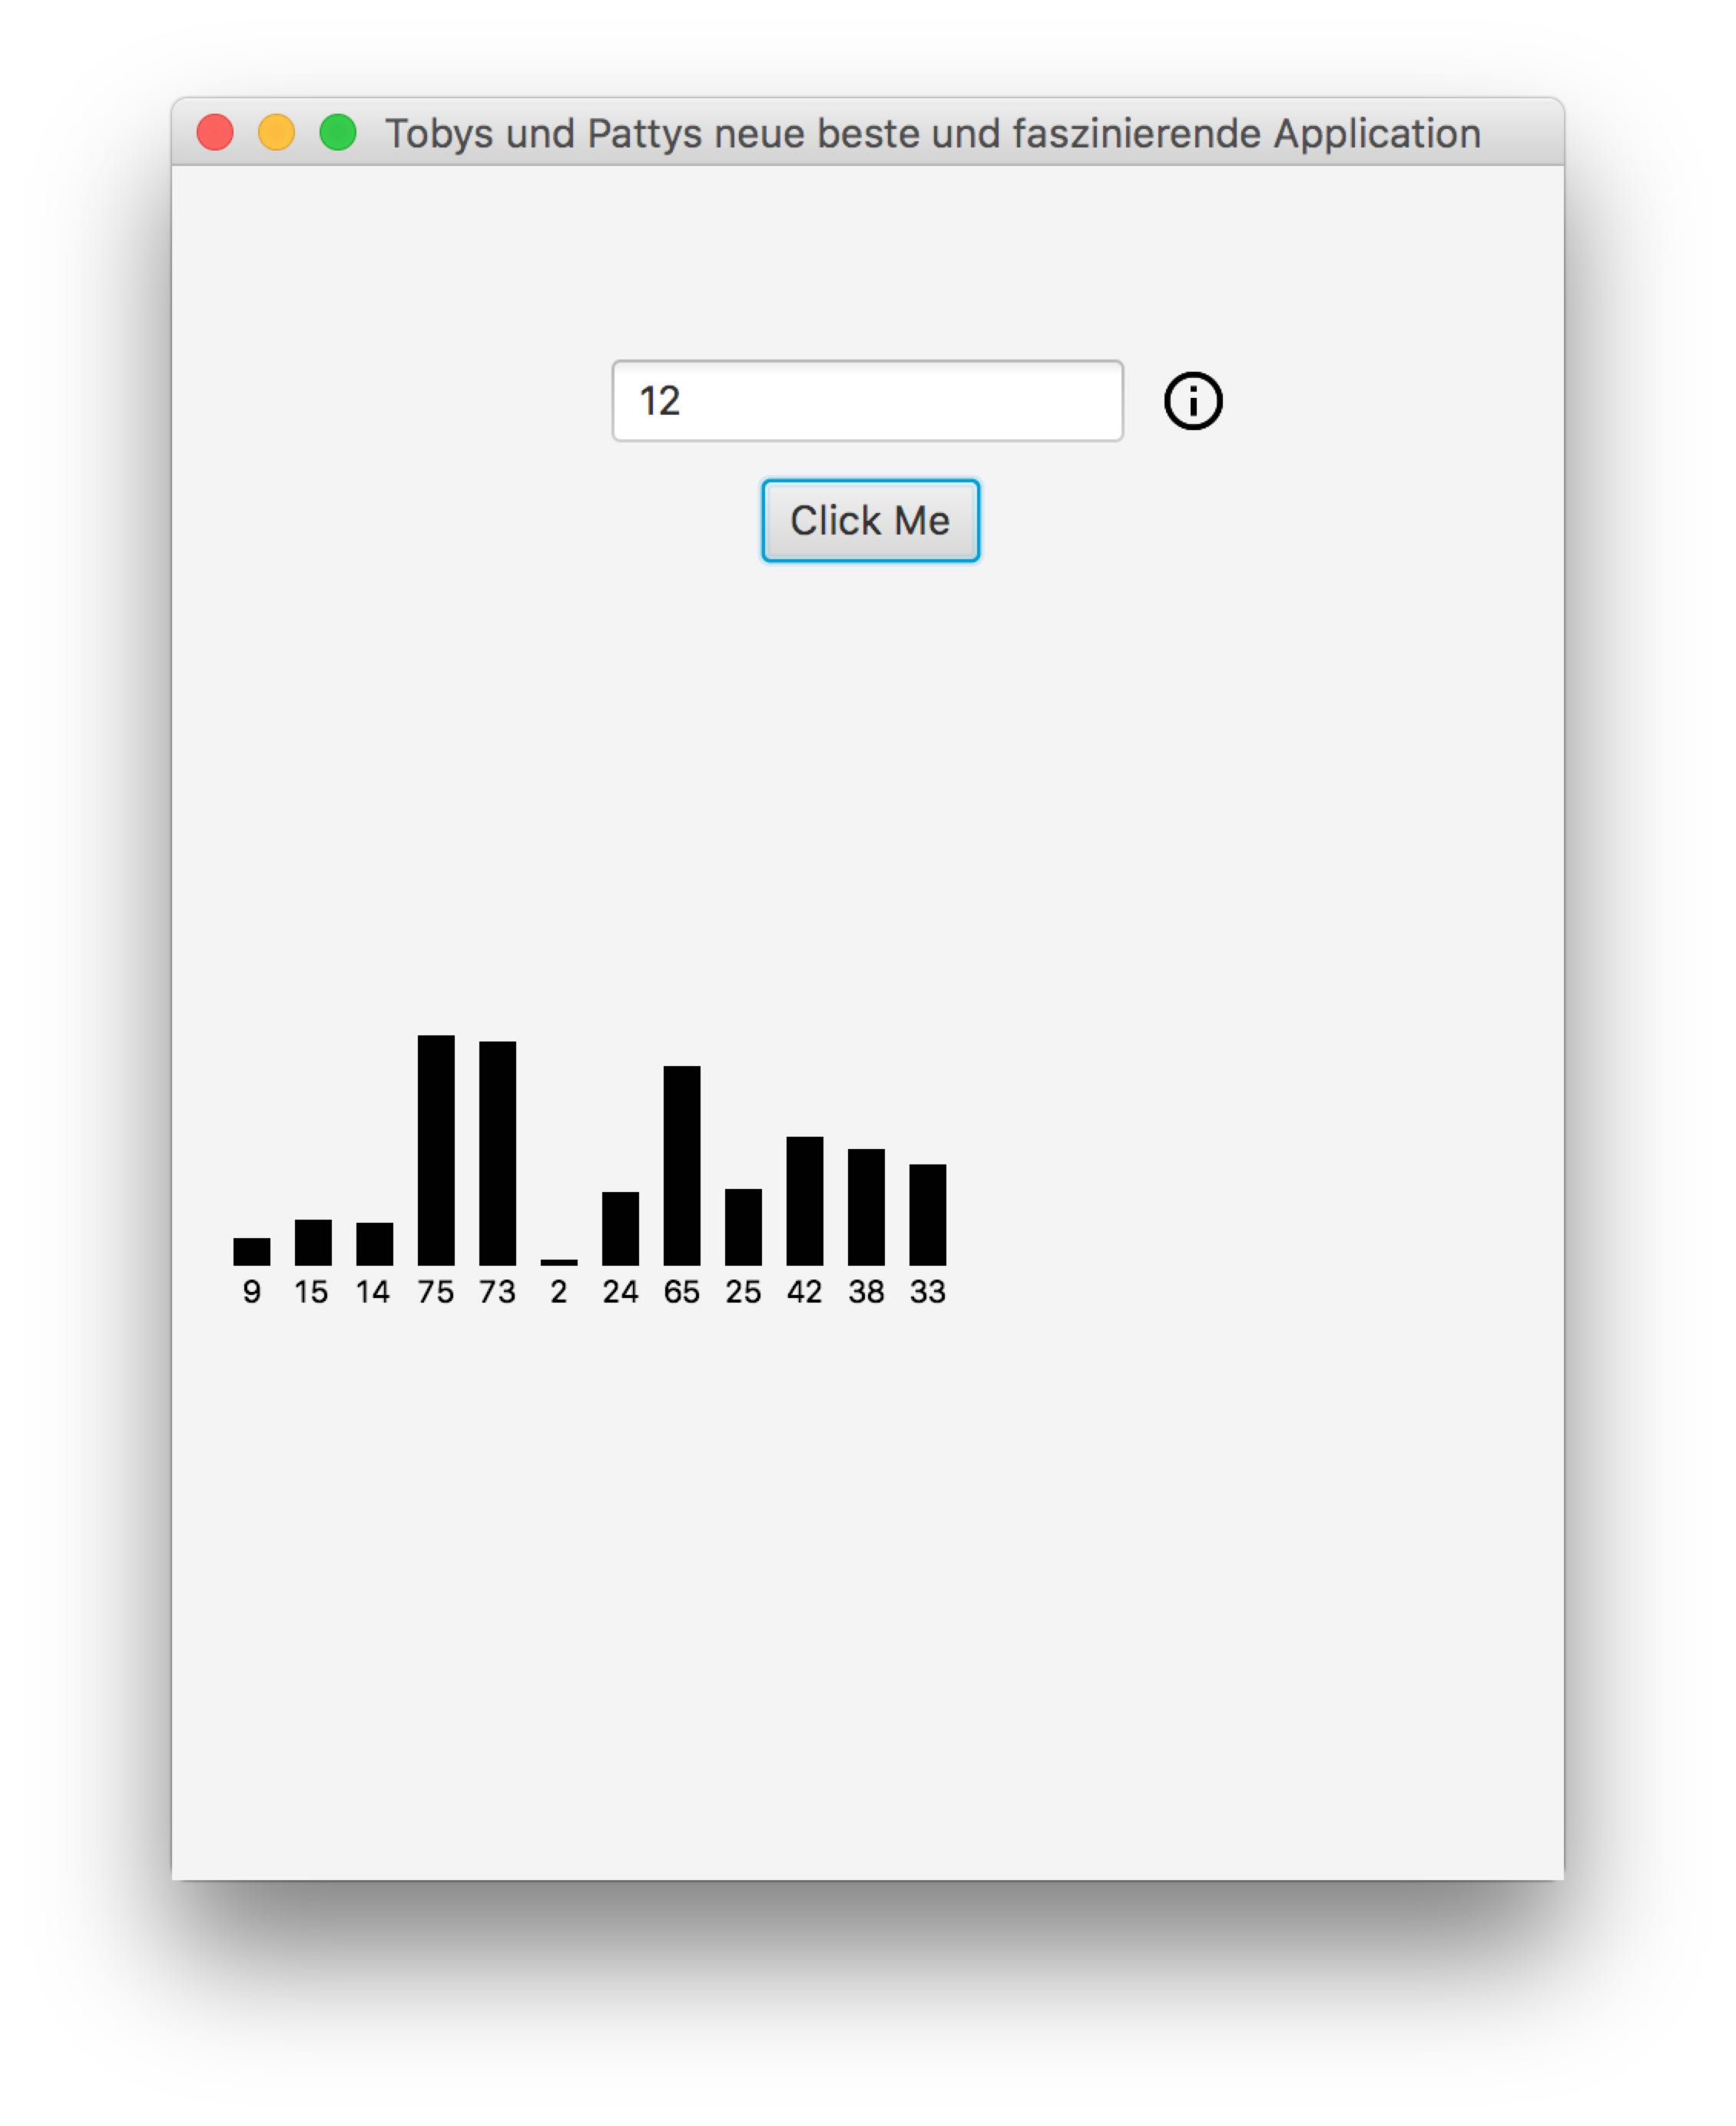
\includegraphics[width=0.55\linewidth]{test-anwendung1}
    \caption{Test Anwendung: Generierung der Balken}
\end{figure}

Außerdem war es eine gute Entscheidung, dass wir uns erst mit einer Anwendung beschäftigten, bei der wir viele Fehler machen konnten, da wir somit keine Design-Entscheidungen im späteren Verlauf bereuen würden.


Das Resultat ist, dass wir selbstbewusst die Beispielanwendung löschten und uns mit einem ausreichend guten Vorwissen an die Entwicklung der eigentlichen Aufgabe machten. Wir wussten nun, wie man auf Events reagiert, wie man Elemente in FXML definiert und in dem Controller anspricht. Wir konnten Elemente nun manipulieren (zwar auf einem \texttt{Canvas}) und kannten uns nun besser mit der baumartigen Struktur von JavaFX aus, bei der oben die \texttt{Stage}, darunter die \texttt{Scene} und darunter die \texttt{Node}s waren.


\begin{figure}[!htb]
    \centering
      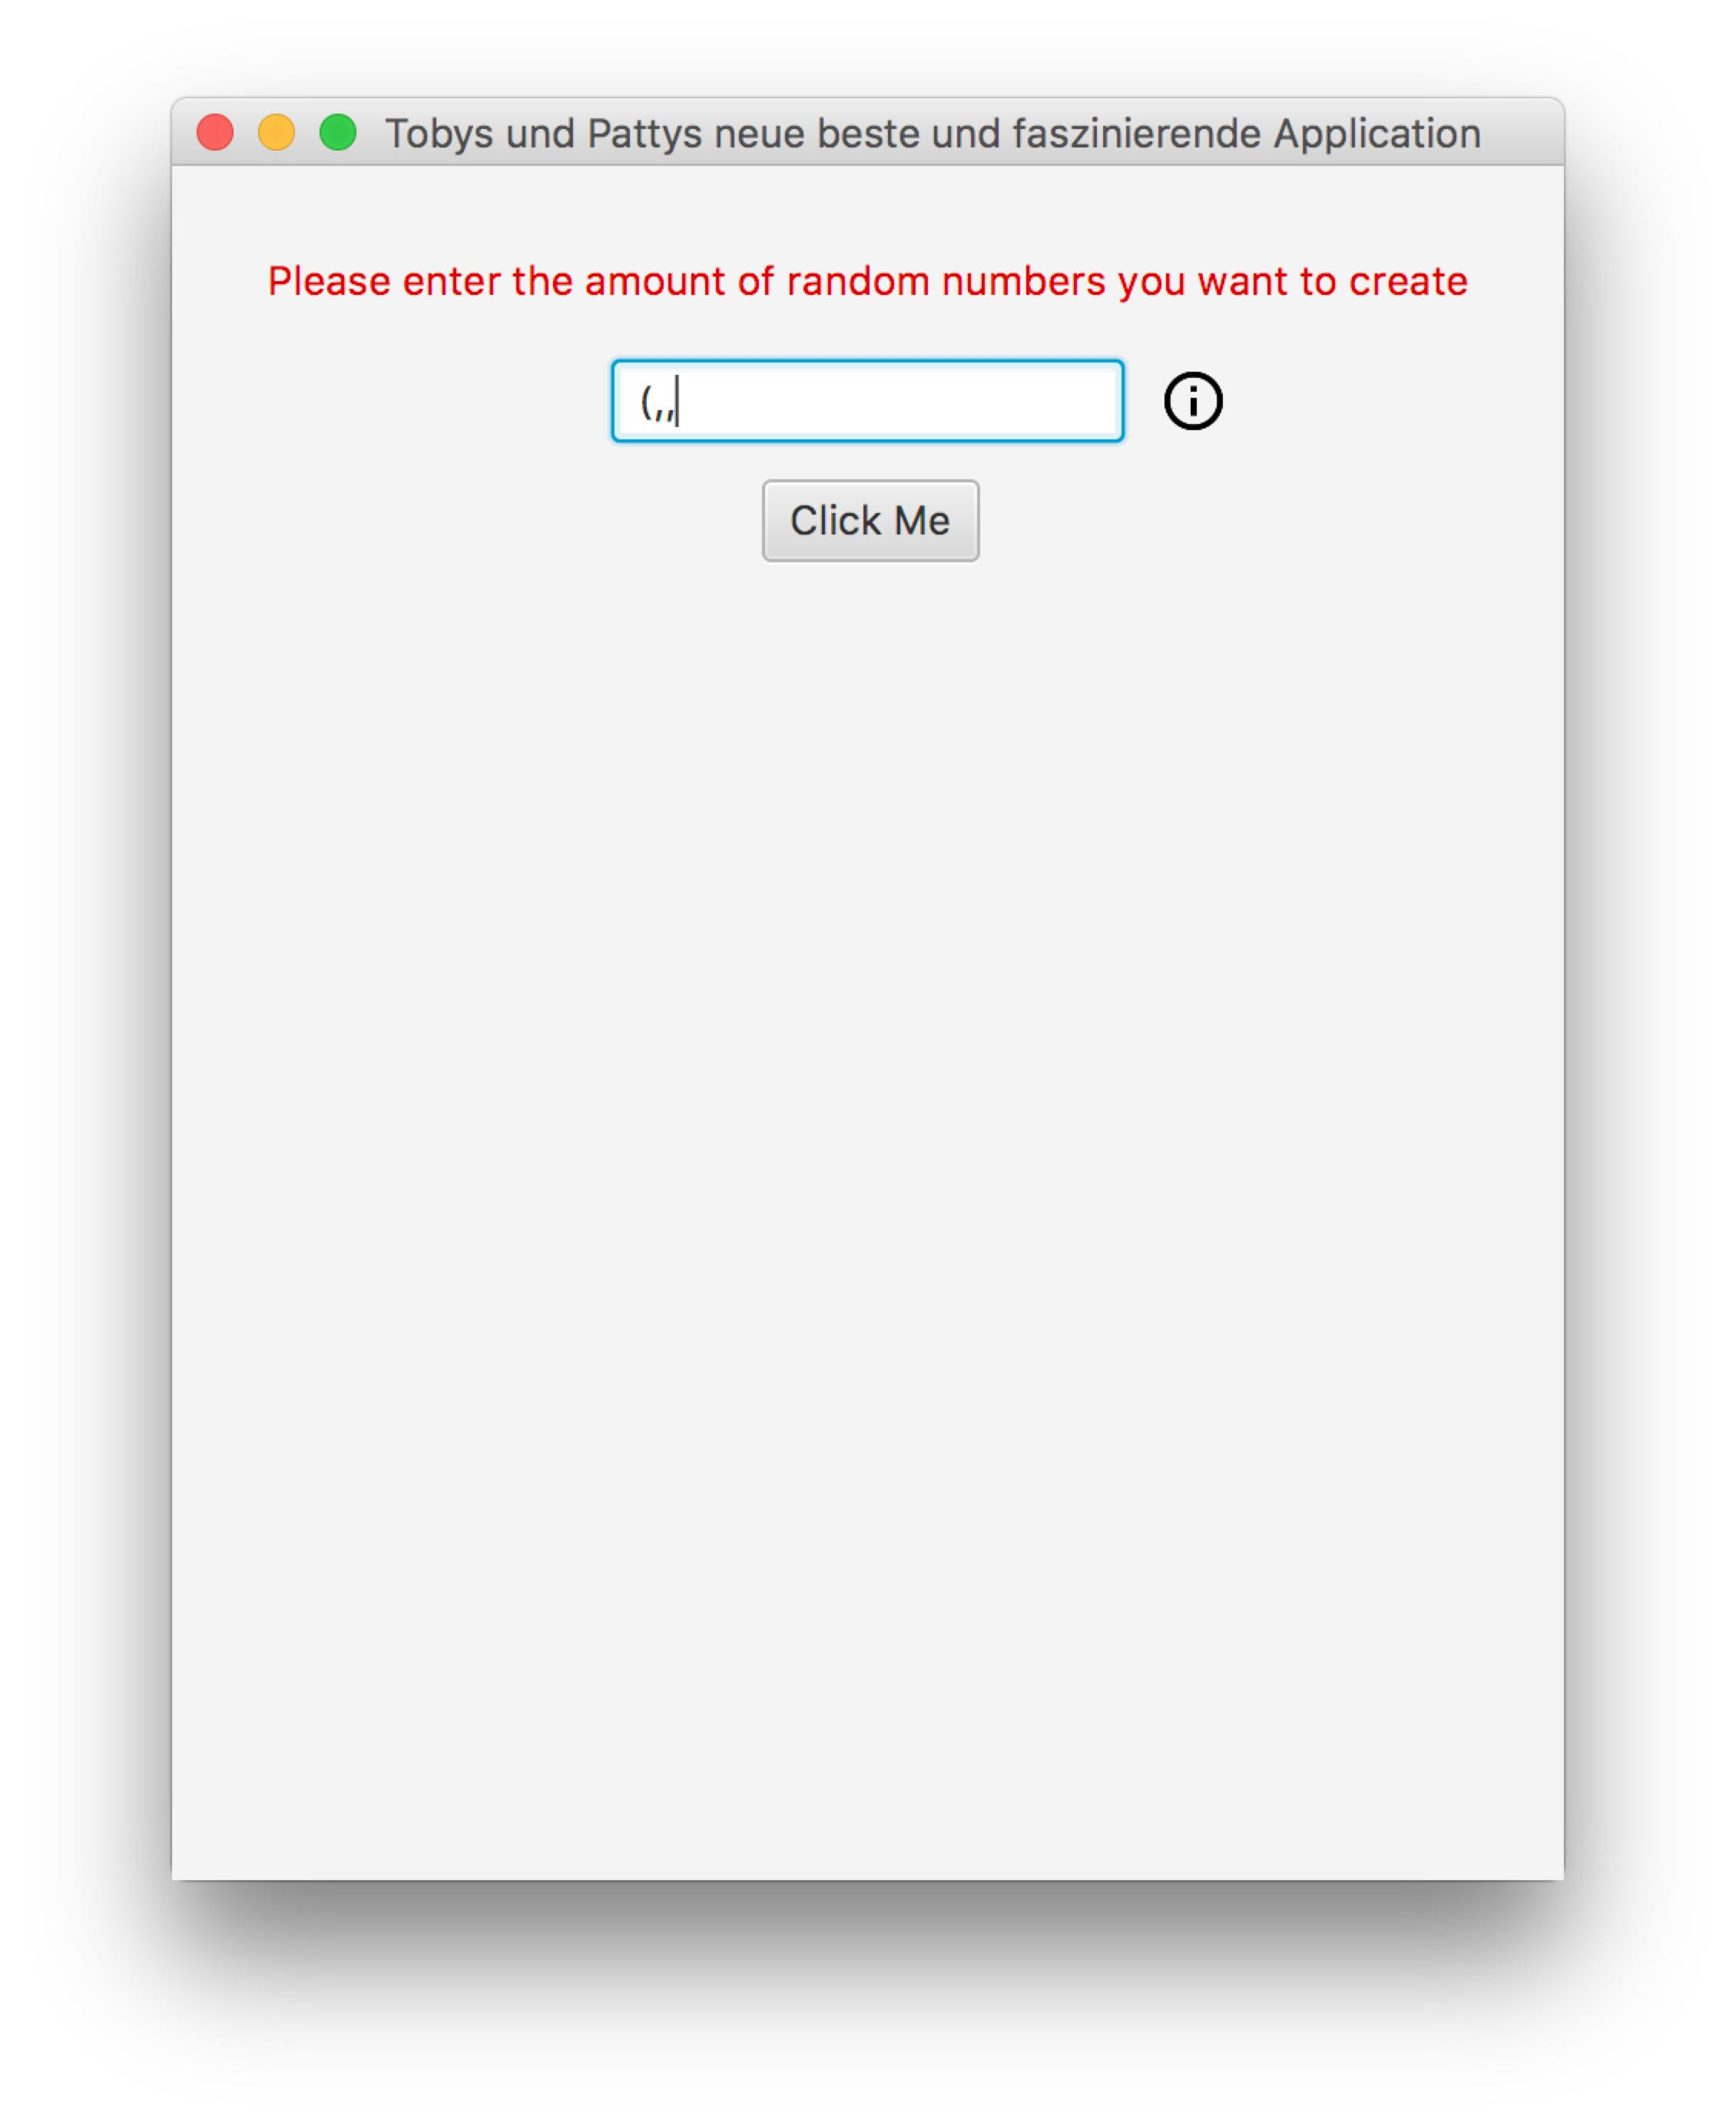
\includegraphics[width=0.55\linewidth]{test-anwendung2}
    \caption{Test Anwendung: Fehlermeldung bei Falscheingabe}
\end{figure}

\subsubsection{Gemeinsame Entwicklung}
Danach haben wir uns täglich getroffen und gemeinsam an der Anwendung gearbeitet. Hierbei haben wir die meiste Zeit vor einem Bildschirm gesessen und gemeinsam entwickelt. Dies hat sich als sehr sinnvoll herausgestellt, da man so schneller Fehlern vorbeugen konnte und wir kleine Probleme diskutieren konnten, ohne den anderen aus Gedanken reißen zu müssen, was eher passiert, wenn jeder an seinem Teil entwickelt. Somit nutzten wir die ganzen Vorteile von \textit{Pair Programming}\footnote{\url{https://www.agilealliance.org/glossary/pairing/}}

\begin{itemize}
\item Wir haben besseren Code geschrieben
\item Wir kannten alle Code-Teile und konnten so Bugs schneller finden und fixen
\item Wir haben viel diskutieren können
\end{itemize}

Im späteren Verlauf wurden einzelne Teile vermehrt aufgeteilt, da es sich hierbei um \textit{einfach zu schreibenden} Code handelte oder weil es zeitlich sinnvoller war, die Arbeit aufzuteilen. Beispielsweise wurden die Shortcuts im Menü eingefügt, während der andere sich über ein bestehendes Problem informierte.

Wir erreichten, was man nur selten bei Abschluss eines Projekts behaupten kann: Eine gerechte Arbeitsteilung, bei der am Ende niemand von sich beansprucht, dass er mehr als der andere gemacht hat.
\section{Kritische Betrachtung}\label{sec:kritische-betrachtung}
Wir haben viele unserer gewünschten Ideen in das Programm implementiert und einige Features sind dazu gekommen, von denen wir es nicht erwartet hatten, dass sie überhaupt möglich sein werden. Es ist aber auch eine Sache weggefallen, die wir sehr gerne implementiert hätten.

\subsection{Erwartete Features}
Wir haben uns zu Beginn viele Gedanken gemacht, wie wir das Programm entwickeln werden und welche Features enthalten sein sollen und müssen. Dabei lagen uns die folgenden ganz besonders am Herzen:

\subsubsection{Elemente als Balken}
Da die Aufgabe die \textbf{Visualisierung} des Algorithmus' war, gab es keinen Zweifel, dass die Elemente nicht einfach als Zahl dargestellt werden können, sondern die Gewichtung auch sichtbar sein soll. Wir haben uns somit dafür entschieden, dass wir diese Gewichtung durch Balken darstellen. Dennoch sollte es einfach sein, die Werte zu vergleichen, damit der Algorithmus immer noch leicht verständlich bleibt.

Durch unsere Klasse \texttt{SortElement}, die von \texttt{Group} erbt, welche wiederum ein Node ist, konnten wir genau das erreichen. Wir hatten ein Objekt, das wir in Gruppen stecken, bewegen, färben und vergleichen konnten. Somit wurde der Code nicht nur lesbarer, sondern die Implementierung auch sehr vereinfacht und ein Nutzer der Anwendung bekommt die Gewichtung von Zahlen mit.

\subsubsection{Einstellbare Anzahl an Elementen}
Um das Programm für den User ansprechend und auch interaktiv zu machen, wollten wir auf jeden Fall die Anzahl an Elementen einstellbar machen. Wir dachten zwar ursprünglich an ein Textfeld, in das der User eine Zahl eingeben kann, jedoch hat man dabei das Problem, dass man die Eingabe auf die folgenden Dinge prüfen muss:

\begin{itemize}
\item Ist der eingegebene String eine Zahl?
\item Erlaubt man auch Double Werte, also Zahlen mit Komma?
\item Wie kennzeichnet man den erlaubten Wertebereich?
\end{itemize}

Aufgrund dieser Probleme haben wir uns nach Alternativen umgesehen und mit dem \texttt{Slider} die perfekte Alternative gefunden, die unseren Ansprüchen genügte und die oben genannten Probleme auf eine sehr intuitive Weise löst.

\subsubsection{Anzahl an Threads}
Wir wollten auch, dass der User die Möglichkeit hat, die Anzahl an Threads einzustellen. Auch hier entschieden wir uns für einen \texttt{Slider}, da die oben beschriebenen Probleme auch bei der Auswahl an Threads existieren. In der jetzigen Form gibt es die Möglichkeit zwischen einem und zwei Threads zu wählen, wieso es nur diese beiden Möglichkeiten gibt, möchten wir in Section \ref{sec:probleme-mit-aktoren} erläutern.

\subsubsection{Zufällig gewählte Elemente erzeugen}
Uns war klar, dass auf irgendeine Art die Elemente erzeugt werden müssen, die dann sortiert werden. Diese Elemente sollten zufälllig generiert werden.

\subsubsection{Sortierung durch Animationen}
Um den Algorithmus zu veranschaulichen, sollten die Elemten aufgespalten und wieder gemerget, also zusammengeführt werden. Diese Schritten sollten durch \textit{herumfliegende} Elemente klar erkennbar sein, wofür sich die JavaFX Transitions anbieten.

\subsubsection{Text-Ausgabe über das, was gerade passiert}
Um den Algorithmus nicht nur visuell zu erklären, wollten wir, dass der User \textit{textuell} darüber informiert wird, was gerade passiert und mit welchen Elementen.

\subsection{Hinzugekommene Features}
Während der Entwicklung merkt man oft, welche essentiellen Features noch fehlen, welche teilweise leicht implementiert werden können oder aber die Nutzbarkeit der App wesentlich verbessern.
\subsubsection{Generierung von vorsortierten Elementen}
Die Generierung von vorsortierten Elementen ist ein Beispiel für eine Feature, das schnell implementiert war, aber die Nutzung der Applikation interessanter macht. Da man durch dieses Feature ein für den Algorithmus typisches Verhalten gut beschreiben kann, haben wir uns entschieden, dass Elemente optionalerweise \textit{sortiert} und \textit{invers sortiert} generiert werden können.

\subsubsection{Interaktive Eingabe von Elementen}
Dieses Feature haben wir implementiert, um unser Programm besser testen zu können. Da man teilweise nicht nur zufällig generierte Zahlen testen möchte, sondern ganz Bestimmte, haben wir uns dazu entschieden, dass man die Elemente durch einen Dialog eingeben kann. Diese müssen dann jedoch auf Zulässigkeit geprüft werden und im Anschluss erzeugt werden. Dieses Feature hat sich nicht nur für Testzwecke als praktisch erwiesen, sondern auch für den \textit{produktien} Einsatz und ist deshalb nun Bestandteil der Anwendung.

\subsubsection{Autoscrolling}
Dieses Feature hat uns viel Zeit gekostet, aber hat sich im Endeffekt gelohnt. Wir haben uns gedacht, dass ein interaktiv zu benutzendes Programm zwar toll ist und dass man von dem User erwarten kann, dass er auf der Pane scrollt, jedoch haben wir es als störend empfunden, dass man das Programm nicht \textit{einfach laufen lassen} konnte. Man musste immer aktiv eingreifen um zu der Stelle zu gelangen, an der der Algorithmus gerade arbeitet. Dies war vor allem bei sehr vielen Elementen anstrengend.

Wir haben aber mit Einschränkungen leben müssen. Bei zwei Threads ist das Autoscrolling nur wirklich nutzbar, wenn die Anzahl an Elementen gerade ist, da das Autscrolling sonst dafür sorgt, dass die Pane immer zum aktiven Geschehen scrollen möchte, was jedoch an zwei verschiedenen Orten ist. Das Resultat ist, dass man von dem Algorithmus nichts mehr mitbekommt. Deswegen haben wir das Feature für zwei Threads bei einer ungeraden Anzahl von Elementen deaktiviert.

\subsubsection{Play, Pause und die Animationsgeschwindigkeit}
Unsere App sticht durch das Feature hervor, dass man die Animationen pausieren und wieder starten kann. Dadurch kann man, beispielsweise bei der Präsentation auf Eigenarten des Algorithmus' hinweisen und an eine andere Stelle scrollen. Das Einstellen der Geschwindigkeit macht die Benutzung der Applikation erst so richtig spannend, denn teilweise möchte man an einen Punkt gelangen und kann es nicht erwarten, bis das Programm da ist. Wenn man diesen Punkt dann erreicht hat, dann möchte man das Geschehen jedoch genau verfolgen und die Geschwindigkeit runter stellen. Genau das haben wir durch den Geschwindigkeits-Slider erreicht und freuen uns auch, dass dieses Feature stabil und verlässlich funktioniert.

\subsubsection{Ein-- und Ausblenden der Leisten}
Das Ein-- und Ausblenden der Logging-Konsole und der Controls ist kein wichtiges Feature, ist aber sehr zweckdienlich, wenn man sich auf die Visualisierung des Algorithmus beschränken möchte. Gerade dadurch, dass die Rekursion durch Verschieben nach unten visualisiert wird und die Bildschirmhöhe begrenzt ist, kann man so mehr auf dem Bildschirm darstellen.

\subsubsection{Shortcuts}
Wir benutzen Shortcuts, um ohne umständliche Navigation die Visualisierung zu starten. Gerade für Präsentationszwecke ist dies sehr praktisch und auch während unserer Tests haben wir gemerkt, wie praktisch es ist, wenn man über die Eingabe zweier Befehle die Animation starten kann. Somit haben wir uns dafür entschieden, alle Menüpunkte mit Shortcuts zu versehen, da dadurch die Nutzung der Anwendung spielerisch wird.

\subsection{Fehlende Features}
Natürlich spielt der Faktor Zeit eine Rolle, wenn man eine solche Anwendung schreibt. Jedoch hat uns auch JavaFX einige Probleme bereitet, die dazu geführt haben, dass wir nicht alles so implementieren konnten, wie wir es gerne wollten. Wir möchten im Folgenden die Punkte nennen, die wir gerne noch implementiert hätten und auf die wir leider verzichten mussten.

\subsubsection{Actors}\label{sec:probleme-mit-aktoren}
Aktoren (im engl. \textit{Actors}) ist ein Modell, das es erlaubt multithreading-fähige Anwendungen zu schreiben. Es handelt sich bei den Aktoren um eine Abstraktions-Schicht, die auf Threads aufbaut. Bei den Aktoren werden unveränderliche (\textit{immutable}) Nachrichten verschickt, auf die reagiert wird. Da wir den Mergesort-Algorithmus multithreading-fähig implementieren sollten, hatten wir uns fest vorgenommen, dass wir die Nebenläufigkeit mittels Aktoren implementieren. Hierbei sollte jeder Actor (also jeder Thread) eine Teilliste bekommen und sortieren. Das Mergen dieser sortierten Listen sollte dann durch eine \texttt{Synchronisation} geschehen. Die Nachricht zwischen den Aktoren wäre die Liste gewesen, die erst unsortiert und später sortiert zwischen den Aktoren ausgetauscht wird.


Diese Implementierungsstrategie ist intuitiv und stabil. Leider hat uns an dieser Stelle JavaFX im Stich gelassen. Die Manipulation der Elemente auf der Pane und das Starten der Transitionen ist leider nicht möglich, man bekommt eine Exception wenn man aus einem anderen Thread auf die Pane zugreifen möchte. Unser Programm nutzte leider von Grund auf den Ansatz, dass man Elemente auf der Pane verschiebt. Somit konnten wir keine Aktoren für die Berechnung und anschließende Animation benutzen. Da wir sehr lange probiert haben, das Aktorenmodell zu nutzen und zum Laufen zu bringen, mussten wir das parallele Ablaufen das Animation durch das mehrfache Abspielen zweier Animations-Sequenzen implementieren. Somit konnten wir uns jedoch auch nur auf zwei Threads konzentrieren.


\subsubsection{Autoscrolling der Logging--Konsole}
Das Autoscrolling in der Logging--Konsole ist zwar vorhanden, aber alles andere als stabil. Dies hat mit einem Fehler in JavaFX zu tun, das beim Ändern des Texts automatisch an die Position 0.0, also den Anfang scrollt. Da wir jedoch mit dem Text-\texttt{Property} arbeiten mussten, um die Darstellung während der Animation zu ermöglichen, mussten wir Werte finden, an denen man an das Ende Scrollen kann, nachdem an die Position 0.0 gesprungen wurde. Wir nutzen momentan eine \texttt{TextArea}, haben eine Implementierung sowohl über ein \texttt{TextFlow} als auch einen \texttt{ListView} versucht. Keine der Lösungen hat funktioniert und somit muss man sich nun mit einer etwas unrund scrollenden Logging--Konsole abfinden. Wir haben entschieden, dass diese Funktionalität keine Prioriät hat.

\subsubsection{Merge: Einfliegen von ursprünglicher Position}
Die Bestimmung der Positionen auf einer \texttt{Pane} ist nicht immer klar und somit mussten wir uns teilweise damit behelfen, dass wir Werte durch das Testen heraus bekommen oder, dass wir Features nicht zu unserer vollen Zufriedenheit implementieren. Ein Beispiel ist das Mergen. Hierbei kommen die Elemente zwar aus der richtigen Richtung, jedoch nicht von der richtigen Position. Dieses Problem hat uns ganze Tage geraubt, es ist nicht möglich die x--Position eines Elements genau zu bestimmen. Weder die absolute Position, noch die relative Position konnte bestimmt werden. Wir mussten es dann darauf beruhen lassen, dass man erkennt, ob ein Element aus der linken, oder der rechten Gruppe kommt.

\section{Fazit}\label{sec:fazit}
Das Projekt war herausfordernd und spannend. Wir haben viele neue Dinge gelernt und besonders die Team--Arbeit hat sich als sehr wertvoll herausgestellt.

Wir sind beide begeistert von der Programmiersprache Scala, die anfangs zwar etwas kompliziert erscheint, aber bei längerer Benutzung wirklich viele praktische Features mitbringt. Viele davon haben wir in dieser Ausarbeitung bereits vorgestellt. Wir empfehlen auf jeden Fall, dass man sich genauer mit dieser Sprache befasst, da besonders die funktionale Programmierung ein sehr interessanter Ansatz ist, die Bibliotheks--Unterstützung durch die Integration in die JVM (und somit Java) sehr gut ist und man nicht unnötig viel Code schreiben muss. Java--Code wirkt im Vergleich mittlerweile umständlich und oft unnötig.

JavaFX, das wir durch ScalaFX genutzt haben, ist \textit{die} neue Bibliothek, die man zur Entwicklung von Benutzeroberflächen nutzt. Als Bestandteil von Java 8 wird diese vermutlich noch lange weiterentwickelt werden. Dass wir uns während dieser Projektarbeit intensiv mit diesem Framework auseinander gesetzt haben, wird sich spätestens dann auszahlen, wenn wir das nächste Mal eine Anwendung mit einer Oberfläche entwickeln werden.

Die Arbeit mit einem richtigen Build--Tool wie \texttt{sbt} und einem Versionskontrollsystem (\texttt{git}), hat von uns verlangt, dass wir uns nicht nur mit der Programmiersprache und Entwicklungsumgebung auseinander setzen, sondern auch die anderen Aspekte, mit denen sich ein Programmierer auseinander setzen muss, kennenlernen.

Was uns überrascht hat, ist die Tatsache, dass die Entwicklung des Algorithmus' nicht nur elementare Kenntnis des Verhaltens vorraussetzte: Man musste alle Aspekte des Algorithmus' verstehen, um sich darüber unterhalten zu können, wie man den Algorithmus nun am besten visualisiert.\\
Somit wurde das sehr theoretische Konzept sehr schnell etwas, das man benannt hat (\texttt{merge}, \texttt{split}, \texttt{sort}, \texttt{shuffle}) und bei dem man dann wusste wie es geschieht. Sehr schnell wurde so aus einem abstrakten Problem ein gestalterisches, bei dem man die Konzepte, die man nun benennen konnte, visuell so präsentieren musste, dass auch jemand, der den Mergesort--Algorithmus nicht kennt, versteht, worum es geht.

Neben all dem technischen Know-How, das wir erworben haben, hat sich aber auch vor allem herausgestellt, wie Zusammenarbeit funktioniert und wie man sich verhält, wenn man auf einmal nicht mehr alles selber macht. Wir haben festgestellt, dass Kommunikation das A und O bei einem erfolgreichen Projekt ist. Da wir mit viel Begeisterung bei der Sache waren und die Entwicklung nicht nur zeitintensiv, sondern auch interessant, lehrreich und unterhaltsam war, blicken wir zufrieden auf das Resultat: Unser Visual-Mergesort.

\clearpage

\addcontentsline{toc}{chapter}{Literatur}
\bibliography{sources}
\bibliographystyle{alpha}
\end{document}
